%%%%%%%%%%%%%%%%%%%%%%%%%%%%%%%%%%%%%%%%%%%%%%%%%%%
%return
%  New template code for TAMU Theses and Dissertations starting Fall 2012.  
%  For more info about this template or the 
%  TAMU LaTeX User's Group, see http://www.howdy.me/.
%
%  Author: Wendy Lynn Turner 
%
%%%%%%%%%%%%%%%%%%%%%%%%%%%%%%%%%%%%%%%%%%%%%%%%%%%

\documentclass[12pt]{report}
\usepackage[letterpaper]{geometry}
\geometry{verbose,tmargin=1.25in,bmargin=1.25in,lmargin=1.4in,rmargin=1.15in}
 \usepackage[doublespacing]{setspace}
 \usepackage{tocloft}
 \usepackage[rm, tiny,center, compact]{titlesec}
 \usepackage{indentfirst}
 \usepackage{etoolbox}
\usepackage{tocvsec2}
 \usepackage[titletoc]{appendix}
 \usepackage{appendix}
% \usepackage{tamuconfig}
 \usepackage{pvamuconfig}
\usepackage{rotating}


\usepackage{lipsum}
\usepackage{multirow}

%\usepackage{fancyhdr}

\newcommand\blfootnote[1]{%
  \begingroup
  \renewcommand\thefootnote{}\footnote{#1}%
  \addtocounter{footnote}{-1}%
  \endgroup
}

% Change the default page style to upper-righter page number
\usepackage{etoolbox}% http://ctan.org/pkg/etoolbox
\patchcmd{\chapter}% <cmd>
  {plain}% <search>
  {myheadings}% <replace>
  {}{}% <success><failure>

\usepackage{algorithm}
%\usepackage{algorithmic}
\usepackage{algpseudocode}

% Added to fix issues with pdf searching in some versions of LaTeX
%\usepackage[T1]{fontenc}\usepackage{lmodern}
%%%%%%%%%%%%%%%%%%%%%%%%%%%%%
\usepackage{float}
\usepackage{listings}
\usepackage{color}
\definecolor{gray}{rgb}{0.4,0.4,0.4}
\definecolor{darkblue}{rgb}{0.0,0.0,0.6}
\definecolor{cyan}{rgb}{0.0,0.6,0.6}

\lstset{
  basicstyle=\ttfamily,
  columns=fullflexible,
  showstringspaces=false,
  commentstyle=\color{gray}\upshape
}

\lstdefinelanguage{XML}
{
  morestring=[b]",
  morestring=[s]{>}{<},
  morecomment=[s]{<?}{?>},
  stringstyle=\color{black},
  identifierstyle=\color{darkblue},
  keywordstyle=\color{cyan},
  morekeywords={xmlns,version,type}% list your attributes here
}

\usepackage{pbox}

%\usepackage{caption}
\usepackage[labelsep=period]{caption}
\usepackage{subcaption}
\usepackage{breakcites}
\usepackage{url}
\usepackage{tabularx}

\usepackage{array}
\newcolumntype{L}[1]{>{\raggedright\let\newline\\\arraybackslash\hspace{0pt}}m{#1}}
\newcolumntype{C}[1]{>{\centering\let\newline\\\arraybackslash\hspace{0pt}}m{#1}}
\newcolumntype{R}[1]{>{\raggedleft\let\newline\\\arraybackslash\hspace{0pt}}m{#1}}

\usepackage{textcomp}
\usepackage{adjustbox}
\usepackage{blindtext}

\usepackage{amsfonts}

%for formating
\usepackage[document]{ragged2e}




%\usepackage{pvamuconfig}
%\usepackage{rotating}

%\usepackage{fancyhdr}
%\fancypagestyle{plain}{%
%\renewcommand{\headrulewidth}{0pt}%
%\fancyhf{}%
%\rhead{\thepage}%
%}


\usepackage{amsthm}


% Hyperref setup below.  You should be able to get away with using uncommenting just the first line.
%\usepackage[hidelinks]{hyperref}

% if \usepackage[hidelinks]{hyperref} doesn't work try this.
% \usepackage{hyperref}  % Hidelinks is an option that removes link visiability.  TAMU Thesis Offices prefers to not see the links. But often doesn't work.  
% 
% \hypersetup{
%     colorlinks=true,
%     linkcolor=black,
%     citecolor=black,
%     filecolor=black,
%     urlcolor=black,
% }
%%%%%%%  End of hyperref setup.  One of these two options should work, but my motto with hyperref is when in doubt, comment it out!
%%%%%%%%%  This hopefully fixes the problem with vertical spacing of section headings at the top of the page..  Commented out in 1.0.7
% \preto\section{%
% \ifnum\value{section}>0\addtocontents{toc}{\vskip-6pt}\fi
% }
% \preto\subsection{%
% \ifnum\value{subsection}=0\addtocontents{toc}{\vskip-6pt}\fi
% \ifnum\value{subsection}>0\addtocontents{toc}{\vskip-6pt}\fi
% } 
%%%%%%%%%%%%%%%%%%%%%%%%%%%%%%%%%%%%%%%%%%%%%%%%%%%%%%



\begin{document}

% Change to PVAMU format
\ifx true false 
\renewcommand{\tamumanuscripttitle}{Demand forecasting using Recurrent neural networks on Smart Meter data}
\renewcommand{\tamupapertype}{Dissertation}
\renewcommand{\tamufullname}{Ishan Khatri}
\renewcommand{\tamudegree}{Master Degree}
\renewcommand{\tamuchairone}{Dr. Lijun Qian}
% Uncomment out the next line if you have co-chairs.  You will also need to edit the titlepage.tex file.
%\newcommand{\tamuchairtwo}{Additional Chair Name}
\renewcommand{\tamumemberone}{Dr. Lijun Qian}
\newcommand{\tamumembertwo}{Dr. Lei Huang}
\newcommand{\tamumemberthree}{Dr. Xiangfang Li}
\renewcommand{\tamudepthead}{Dr. Pamela Obiomon}
\renewcommand{\tamugradmonth}{Aug}
\renewcommand{\tamugradyear}{2017}
\renewcommand{\tamudepartment}{Department of Electrical and Computer Engineering}
\fi

\renewcommand{\pvamucollege}{PRAIRIE VIEW A\protect\&M UNIVERSITY\protect\\COLLEGE OF ENGINEERING\protect\\PRAIRIE VIEW, TEXAS}
\renewcommand{\pvamumanuscripttitle}{Demand forecasting using convolutional neural networks on big real world data}
\renewcommand{\pvamupapertype}{Thesis}
\renewcommand{\pvamusubmitto}{Submitted to the Graduate School\\In Partial Fulfillment of the Requirements for\\The Degree of}
\renewcommand{\pvamudegree}{MASTER OF SCIENCE}
\renewcommand{\pvamumajor}{ELECTRICAL AND COMPUTER ENGINEERING}
\renewcommand{\pvamufullname}{Ishan Khatri}
\renewcommand{\pvamuadvisor}{Advisor Name}
\renewcommand{\pvamudepthead}{Department Head}
\renewcommand{\pvamucollegedean}{College Dean Name}
\renewcommand{\pvamugraddean}{Graduate School Dean Name}
\renewcommand{\pvamugradmonth}{Aug}
\renewcommand{\pvamugradyear}{2017}


%%%%%%%%%%%%%%%%%%%%%%%%%%%%%%%%%%%%%%%%%%%%%%%%%%%%
%
%  New template code for TAMU Theses and Dissertations starting Fall 2012.  
%  For more info about this template or the 
%  TAMU LaTeX User's Group, see http://www.howdy.me/.
%
%  Author: Wendy Lynn Turner 
%	 Version 1.0 
%  Last updated 8/5/2012
%
%%%%%%%%%%%%%%%%%%%%%%%%%%%%%%%%%%%%%%%%%%%%%%%%%%%

%%%%%%%%%%%%%%%%%%%%%%%%%%%%%% 
%% TITLE PAGE
%% The values get updated automatically.  Please do not make changes to this file other than adding/deleting committee members where necessary.
%%%%%%%%%%%%%%%%%%%%%%%%%%%%%%

\providecommand{\tabularnewline}{\\}



\begin{titlepage}
\begin{center}
\MakeUppercase{\tamumanuscripttitle}
\vspace{4em}

A \tamupapertype

by

\MakeUppercase{\tamufullname}

\vspace{4em}

\begin{singlespace}

Submitted to the Office of Graduate and Professional Studies of \\
Prairie View A\&M University \\

in partial fulfillment of the requirements for the degree of \\
\end{singlespace}

\MakeUppercase{\tamudegree}
\par\end{center}
\vspace{2em}
\begin{singlespace}
\begin{tabular}{ll}
 & \tabularnewline
& \cr
% If you have Co-Chairs comment out the 'Chair of Committee' line below and uncomment the 'Co-Chairs of Committee' line.
Chair of Committee, & \tamuchairone\tabularnewline
%Co-Chairs of Committee, & \tamuchairone\tabularnewline & \tamuchairtwo\tabularnewline
Committee Members, & \tamumemberone\tabularnewline
 & \tamumembertwo\tabularnewline
 & \tamumemberthree\tabularnewline
Head of Department, & \tamudepthead\tabularnewline

\end{tabular}
\end{singlespace}
\vspace{3em}

\begin{center}
\tamugradmonth \hspace{2pt} \tamugradyear

\vspace{3em}

Major Subject: \tamudepartment \par
\vspace{3em}
Copyright \tamugradyear \hspace{.5em}\tamufullname 
\par\end{center}
\end{titlepage}
\pagebreak{}




 % This is simply a file that formats and adds your titlepage, please do not edit this unless you have a specific need. .
%%%%%%%%%%%%%%%%%%%%%%%%%%%%%%%%%%%%%%%%%%%%%%%%%%%
%
%  New template code for TAMU Theses and Dissertations starting Fall 2012.  
%  For more info about this template or the 
%  TAMU LaTeX User's Group, see http://www.howdy.me/.
%
%  Author: Wendy Lynn Turner 
%	 Version 1.0 
%  Last updated 8/5/2012
%
%%%%%%%%%%%%%%%%%%%%%%%%%%%%%%%%%%%%%%%%%%%%%%%%%%%

%%%%%%%%%%%%%%%%%%%%%%%%%%%%%% 
%% TITLE PAGE
%% The values get updated automatically.  Please do not make changes to this file other than adding/deleting committee members where necessary.
%%%%%%%%%%%%%%%%%%%%%%%%%%%%%%

\begin{titlepage}
\begin{center}

\vspace*{50 pt}
%\providecommand{\tabularnewline}{\\}
\MakeUppercase{\pvamumanuscripttitle}

\vspace{60 pt}
A \pvamupapertype

by

\MakeUppercase{\pvamufullname}

\vspace{60 pt}

\begin{singlespace}
Submitted to the Office of Graduate Studies of \\
Prairie View A\&M University \\
in partial fulfillment of the requirements for the degree of\\
\end{singlespace}

\vspace{20 pt}
\MakeUppercase{\pvamudegree}

\vspace{60 pt}

%\begin{center}
\pvamugradmonth \hspace{2pt} \pvamugradyear
%\par\end{center}

\vspace{60 pt}

Major Subject: Electrical Engineering
\par\end{center}

\end{titlepage}
\pagebreak{}





%%%%%%%%%%%%%%%%%%%%%%%%%%%%%%%%%%%%%%%%%%%%%%%%%%%
%
%  New template code for TAMU Theses and Dissertations starting Fall 2012.  
%  For more info about this template or the 
%  TAMU LaTeX User's Group, see http://www.howdy.me/.
%
%  Author: Wendy Lynn Turner 
%	 Version 1.0 
%  Last updated 8/5/2012
%
%%%%%%%%%%%%%%%%%%%%%%%%%%%%%%%%%%%%%%%%%%%%%%%%%%%

%%%%%%%%%%%%%%%%%%%%%%%%%%%%%% 
%% TITLE PAGE
%% The values get updated automatically.  Please do not make changes to this file other than adding/deleting committee members where necessary.
%%%%%%%%%%%%%%%%%%%%%%%%%%%%%%

\begin{titlepage}
\begin{center}

\vspace*{12 pt}
\MakeUppercase{\pvamumanuscripttitle}

\vspace{18 pt}
A \pvamupapertype

by

\MakeUppercase{\pvamufullname}

\vspace{18 pt}

\begin{singlespace}
Submitted to the Office of Graduate Studies of \\
Prairie View A\&M University \\
in partial fulfillment of the requirements for the degree of\\
\end{singlespace}

\vspace{12 pt}
\MakeUppercase{\pvamudegree}

\vspace{12 pt}

\end{center}

\begin{singlespace}
\hspace*{1ex} Approved as to style and content by:
\vspace{18 pt}
\newcommand{\specialcell}[2][l]{%
  \begin{tabular}[#1]{@{}l@{}}#2\end{tabular}}

\begin{tabular}{L{8cm} L{8cm} }
       \specialcell{ \underline{\hspace{6cm}} \\Lijun Qian\\Chair of Committee } 
            & \specialcell{ \underline{\hspace{6cm}} \\Lei Huang\\Committee Member }\\
       {} & {} \\
       \specialcell{ \underline{\hspace{6cm}}\\Pamela Obiomon\\Committee Member }
            & \specialcell{ \underline{\hspace{6cm}}  \\Xiangfang Li\\Committee Member } \\
       {} & {} \\
        \specialcell{ \underline{\hspace{6cm}} \\Pamela Obiomon\\Head of Department }
            & \specialcell{ \underline{\hspace{6cm}} \\Kendall T. Harris\\Dean, Roy G. Perry College of Engineering }\\
       {} & {} \\
            \specialcell{ \underline{\hspace{6cm}} \\Cajetan M. Akujuobi\\Dean, Graduate Studies }\\
\end{tabular}

\end{singlespace}
\begin{center}
\vspace{18 pt}
\pvamugradmonth \hspace{2pt} \pvamugradyear \\
\vspace{5 pt}
Major Subject: Electrical Engineering
\end{center}

\end{titlepage}
\pagebreak{}





%%%%%%%%%%%%%%%%%%%%%%%%%%%%%%%%%%%%%%%%%%%%%%%%%%%%
%
%  New template code for TAMU Theses and Dissertations starting Fall 2012.  
%  For more info about this template or the 
%  TAMU LaTeX User's Group, see http://www.howdy.me/.
%
%  Author: Wendy Lynn Turner 
%	 Version 1.0 
%  Last updated 8/5/2012
%
%%%%%%%%%%%%%%%%%%%%%%%%%%%%%%%%%%%%%%%%%%%%%%%%%%%
%%%%%%%%%%%%%%%%%%%%%%%%%%%%%%%%%%%%%%%%%%%%%%%%%%%%%%%%%%%%%%%%%%%%%
%%                           ABSTRACT 
%%%%%%%%%%%%%%%%%%%%%%%%%%%%%%%%%%%%%%%%%%%%%%%%%%%%%%%%%%%%%%%%%%%%%


\chapter*{ABSTRACT}
\addcontentsline{toc}{chapter}{ABSTRACT} % Needs to be set to part, so the TOC doesn't add 'CHAPTER ' prefix in the TOC.

\thispagestyle{plain} % No headers, just page numbers
\pagenumbering{roman} % Roman numerals
\setcounter{page}{3}

\begin{center}

\pvamumanuscripttitle .

(\pvamugradmonth \hspace{2pt} \pvamugradyear)

\vspace{15pt}

\pvamufullname, B.Eng., Lalbhai Dalpatbhai College of Engineering

Chair of Advisory Committee: Dr. Lijun Qian

\par\end{center}

\justify

\indent 
%\justify 

	Demand forecasting has become very significant in recent years because of its accurate and efficient resource allocation for companies. However, demand forecasting usually involves processing very large and sophisticated data sets and it is very challenging to achieve accurate prediction. Although there are many existing methods in the literature, they could not be directly applied to big data. In this thesis, a novel demand forecasting method using deep learning specifically, a Convolutional Neural Network (CNN) based model is proposed to process huge amounts of data. A unique feature of the proposed method is that it has adaptable computational intricacy even with the increasing dimensionality of the data. As a result, the proposed method has excellent scalability. Large data sets, namely the usage data of Bike Sharing Service in New York City are used to validate the proposed method. The goal is to predict hourly bike rental demand in every station of New York City to improve the service and environment, and eventually build a ``Green" city. The results demonstrate the effectiveness and superior performance of the proposed scheme. This is also one of winning strategies of the student team from the CREDIT Center in the 2016 IEEE Big Data Analytics Competition organized by the IEEE Big Data Initiative.

%In modern age and time, the term "Big Data" is one of the most discussed topic. It is also currently a massive challenge with many applications and has become the digital resource to power our real world and is anticipated to continue to do so in foreseeable future. In order to deal with this challenge, the method Machine Learning is becoming more and more popular. This method indicates to automated detection in the data to find meaningful patterns. In this thesis we discuss how can we use Machine learning for doing demand forecasting and propose a model for transportation demand forecasting and results also showes the efficiency of the method. This forecasting is deeply relying on understanding the data and identifying the problem, prospective, confronts and specially related applications.
%
%In order to disseminate knowledge IEEE Big Data Initiative along with CyberC prepared a competition of Big Data analytics where the goal was to increase the usage of Bike Sharing Service in New York City, and the idea of this thesis came from winning the competition which provided the dataset of City Bike share data of New York City. In order to solve the problem I have used historic bike usage with the weather data from another domain and treat those as a time series problem and attempted to compare it with a image processing problem by using Convolutional Neural Network (CNN) in order to forecast hourly bike rental demand in NYC. This thesis absorbed a lot of knowledge from the competition and try to find a model with the lowest error rate. We also then compared our model by building three other very popular baseline methods in order to show the differences in prediction accuracy. This thesis in overall asks a simple question ``How many bikes in every hour can meet users requirement?". In future I would like to treat every station individually and forecast their bike demands separately. Therefore, the truthful meaning of this thesis is to improve the bike share rebalance problem by forecasting the bike demand in hourly basis and to find a way to give the city bike users a better experience overall. 



 

\pagebreak{}








%%%%%%%%%%%%%%%%%%%%%%%%%%%%%%%%%%%%%%%%%%%%%%%%%%%%
%
%  New template code for TAMU Theses and Dissertations starting Fall 2012.  
%  For more info about this template or the 
%  TAMU LaTeX User's Group, see http://www.howdy.me/.
%
%  Author: Wendy Lynn Turner 
%	 Version 1.0 
%  Last updated 8/5/2012
%
%%%%%%%%%%%%%%%%%%%%%%%%%%%%%%%%%%%%%%%%%%%%%%%%%%%

%%%%%%%%%%%%%%%%%%%%%%%%%%%%%%%%%%%%%%%%%%%%%%%%%%%%%%%%%%%%%%%%%%%%%%
%%                           DEDICATION
%%%%%%%%%%%%%%%%%%%%%%%%%%%%%%%%%%%%%%%%%%%%%%%%%%%%%%%%%%%%%%%%%%%%%
\chapter*{DEDICATION}
\addcontentsline{toc}{chapter}{DEDICATION}  % Needs to be set to part, so the TOC doesnt add 'CHAPTER ' prefix in the TOC.



\indent This is an optional page.  Lorem ipsum dolor sit amet, consectetur adipiscing elit. Integer lectus quam, condimentum quis bibendum eu, sollicitudin eget lacus. Praesent non sodales odio. Class aptent taciti sociosqu ad litora torquent per conubia nostra, per inceptos himenaeos. Nulla ac luctus sapien. Morbi cursus sapien eget lorem fermentum hendrerit. Nam ac erat dui, in cursus velit. Vivamus hendrerit porttitor nisi, ut porttitor lorem volutpat eget. In ligula ligula, euismod ut condimentum sit amet, pulvinar sit amet diam. Pellentesque interdum, ipsum ullamcorper consequat dignissim, sem arcu egestas mauris, vitae interdum sem tortor ut ante. Nunc blandit laoreet nisi, non rutrum lorem hendrerit quis. Cras nunc diam, convallis et feugiat at, auctor id libero. Nunc facilisis massa eu eros imperdiet vestibulum. Vestibulum ante ipsum primis in faucibus orci luctus et ultrices posuere cubilia Curae; Donec non velit vitae tortor blandit semper.

Etiam vitae dolor nulla. Ut eros odio, rhoncus eget placerat vitae, elementum ac ante. Proin vitae odio eu nisl pharetra mattis. Pellentesque habitant morbi tristique senectus et netus et malesuada fames ac turpis egestas. Phasellus fermentum lacus consectetur neque consequat ullamcorper. Cras blandit urna non dui consequat molestie. Curabitur viverra nibh at nisi semper faucibus. Nam egestas mauris a enim dignissim nec consectetur tortor rutrum. Mauris at nisi in est luctus congue ut mattis est. Ut pretium, mi quis elementum cursus, ante eros suscipit ligula, ut porttitor elit leo sed turpis. Nam sed dui ligula.


\pagebreak{}

%%%%%%%%%%%%%%%%%%%%%%%%%%%%%%%%%%%%%%%%%%%%%%%%%%%
%
%  New template code for TAMU Theses and Dissertations starting Fall 2012.  
%  For more info about this template or the 
%  TAMU LaTeX User's Group, see http://www.howdy.me/.
%
%  Author: Wendy Lynn Turner 
%	 Version 1.0 
%  Last updated 8/5/2012
%
%%%%%%%%%%%%%%%%%%%%%%%%%%%%%%%%%%%%%%%%%%%%%%%%%%%


%%%%%%%%%%%%%%%%%%%%%%%%%%%%%%%%%%%%%%%%%%%%%%%%%%%%%%%%%%%%%%%%%%%%%%
%%                           ACKNOWLEDGEMENTS
%%%%%%%%%%%%%%%%%%%%%%%%%%%%%%%%%%%%%%%%%%%%%%%%%%%%%%%%%%%%%%%%%%%%%
\setlength{\parindent}{1.5em}
\chapter*{ACKNOWLEDGEMENTS}
\addcontentsline{toc}{chapter}{ACKNOWLEDGEMENTS}  % Needs to be set to part, so the TOC doesnt add 'CHAPTER ' prefix in the TOC.
\thispagestyle{plain} % No headers, just page numbers
%\setlength{\parskip}{1em}
First I would like to thank my Advisor Dr. Lijun Qian, of the Electrical and Computer Engineering department at Prairie View A\&M University. The endless support and opportunity he provided me is unexplainable. The door to Dr.Lijun Qian's  office was always open for me and whenever I faced problems and needed any advice he was always there to steer me to the right direction .

I would also like to thank Dr. Xishuang Dong, Post doc of Electrical engineering department, without his passionate participation and input, this thesis could not have been successfully conducted. 

This research work is supported in part by the U.S. Office of the Assistant Secretary of Defense for Research and Engineering (OASD(R\&E)) under agreement number FA8750-15-2-0119, and by the U.S. Army Research Office under agreement number W911NF-16-1-0496. The U.S. Government is authorized to reproduce and distribute reprints for Governmental purposes notwithstanding any copyright notation thereon. The views and conclusions contained herein are those of the authors and should not be interpreted as necessarily representing the official policies or endorsements, either expressed or implied, of the Office of the Assistant Secretary of Defense for Research and Engineering (OASD(R\&E)), the Army Research Office, or the U.S. Government.

I would also like to thank all the members of the CREDIT (Center of excellence in Research and Education for big military Data InTelligence) center for their support, they have not only helped me with their technical knowledge they are also the most friendly and helpful people I met. 

Finally I would like to thank my parents, my brothers, my sister-in-law, my uncle and aunt who are the only family I have in Texas for their unbelievable contribution and providing unfailing support and encouragement throughout my years of study and the process of researching and writing this thesis. This accomplishment would not have been possible without them. Thank you. 

\pagebreak{}

\ifx true false
\vspace*{\fill}
\begin{center}
A.M.D.G.
\end{center}
\vspace*{\fill}
\pagebreak{}
\fi

%%%%%%%%%%%%%%%%%%%%%%%%%%%%%%%%%%%%%%%%%%%%%%%%%%%%
%
%  New template code for TAMU Theses and Dissertations starting Fall 2012.  
%  For more info about this template or the 
%  TAMU LaTeX User's Group, see http://www.howdy.me/.
%
%  Author: Wendy Lynn Turner 
%	 Version 1.0 
%  Last updated 8/5/2012
%
%%%%%%%%%%%%%%%%%%%%%%%%%%%%%%%%%%%%%%%%%%%%%%%%%%%

%%%%%%%%%%%%%%%%%%%%%%%%%%%%%%%%%%%%%%%%%%%%%%%%%%%%%%%%%%%%%%%%%%%%%%
%%                           NOMENCLATURE
%%%%%%%%%%%%%%%%%%%%%%%%%%%%%%%%%%%%%%%%%%%%%%%%%%%%%%%%%%%%%%%%%%%%%
\addcontentsline{toc}{chapter}{NOMENCLATURE}  % Needs to be set to part, so the TOC doesnt add 'CHAPTER ' prefix in the TOC.

\chapter*{NOMENCLATURE}
\begin{table}
\begin{tabular}{ll}
BBA  & Basic Belief Assignment\tabularnewline
BD & Big Data \tabularnewline
Bel  & Belief\tabularnewline
Bl & Belief (conditional) \tabularnewline
BoE  & Body of Evidence\tabularnewline
CCT   & Conditional Core Theorem\tabularnewline
CF & Common Referencing\tabularnewline
COMINT & Communications Intelligence \tabularnewline
DoD & Department of Defense \tabularnewline
DRC & Dempsters Rule of Combination \tabularnewline
DSmT & Dezert Smarandache Theory \tabularnewline
DST & Dempster-Shafer Theory \tabularnewline
FoD & Frame of Discernment \tabularnewline
FST & Fuzzy-Set Theory \tabularnewline
GEOINT & Geo spatial Intelligence \tabularnewline
HCI &  Human/Computer Interaction \tabularnewline
HUMINT & Human Intelligence \tabularnewline
IW & Indication and Warning \tabularnewline
JDL & Joint Directors of Laboratories \tabularnewline
KF & Kalman Filter \tabularnewline
MASINT & Measurements and signatures Intelligence \tabularnewline
MCMC & Markov-Chain Monte-Carlo \tabularnewline
MSDF & Multi-Sensor data Fusion \tabularnewline
OSINT & Open-source Intelligence \tabularnewline
PCR & Proportional Conflict Redistribution \tabularnewline
Pl & Plausibility \tabularnewline 
RCR & Robust Combination Rules \tabularnewline
RST & Random Set Theory \tabularnewline
SMC & Sequential Monte-Carlo \tabularnewline
SRC & Smet's Rule of Combination \tabularnewline
TBM & Transferable Belief Model\tabularnewline
YRC & Yager's Rule of Combination \tabularnewline
\end{tabular}
\end{table}

%\vspace{2em}


\pagebreak{}

%%%%%%%%%%%%%%%%%%%%%%%%%%%%%%%%%%%%%%%%%%%%%%%%%%%
%
%  New template code for TAMU Theses and Dissertations starting Fall 2012.  
%  For more info about this template or the 
%  TAMU LaTeX User's Group, see http://www.howdy.me/.
%
%  Author: Wendy Lynn Turner 
%	 Version 1.7
%  Last updated 3/24/2014
%
%%%%%%%%%%%%%%%%%%%%%%%%%%%%%%%%%%%%%%%%%%%%%%%%%%%
%%%%%%%%%%%%%%%%%%%%%%%%%%%%%%%%%%%%%%%%%%%%%%%%%%%%%%%%%%%%%%%%%%%%%%
%%       TABLE OF CONTENTS
%%%%%%%%%%%%%%%%%%%%%%%%%%%%%%%%%%%%%%%%%%%%%%%%%%%%%%%%%%%%%%%%%%%%%
% single-space sections in Table of Contents  - commented in version 1.7
%\renewcommand{\cftsecafterpnum}{\vskip0.5\baselineskip}
%\renewcommand{\cftsubsecafterpnum}{\vskip0.5\baselineskip}
%\renewcommand{\cftsubsubsecafterpnum}{\vskip0.5\baselineskip}
%%%%%%%%%%%%%%%%%%%%%%%%%%%%%%%%%%%%%%%%%%%%%%%%%%%

\phantomsection
\addcontentsline{toc}{chapter}{TABLE OF CONTENTS}  

\begin{singlespace}
\renewcommand\contentsname{\normalfont} {\large\bfseries{\centerline{TABLE OF CONTENTS}}}

%\setcounter{tocdepth}{4} % This puts \subsubsection[]{×} in your List of Tables.  The default is 3.


%%%%%%%%%%%%%  Adds Page above the page number in TOC
\setlength{\cftaftertoctitleskip}{1em}
\renewcommand{\cftaftertoctitle}{%
\hfill{\normalfont {Page}\par}}



\tableofcontents

\end{singlespace}

\pagebreak{}

%%%%%%%%%%%%%%%%%%%%%%%%%%%%%%%%%%%%%%%%%%%%%%%%%%%%%%%%%%%%%%%%%%%%%%
%%                           LIST OF FIGURES
%%%%%%%%%%%%%%%%%%%%%%%%%%%%%%%%%%%%%%%%%%%%%%%%%%%%%%%%%%%%%%%%%%%%%

\phantomsection
\addcontentsline{toc}{chapter}{LIST OF FIGURES}  

%\renewcommand{\cftloftitlefont}{\large\bfseries\center\normalfont\MakeUppercase}
\renewcommand{\cftloftitlefont}{\large\bfseries\center\MakeUppercase}

\setlength{\cftbeforeloftitleskip}{-12pt} %% Positions the LOF title vertically to match the chapter titles
\renewcommand{\cftafterloftitleskip}{12pt}


\renewcommand{\cftafterloftitle}{%
\\[4em]\mbox{}\hspace{2pt}FIGURE\hfill{\normalfont Page}\vskip\baselineskip}

\begingroup


\begin{center}
\begin{singlespace}
%% These values make the lof table entries appear double spaced between.
\setlength{\cftbeforechapskip}{0.4cm}
\setlength{\cftbeforesecskip}{0.30cm}
\setlength{\cftbeforesubsecskip}{0.30cm}
\setlength{\cftbeforefigskip}{0.4cm}
\setlength{\cftbeforetabskip}{0.4cm} 

\listoffigures

\end{singlespace}
\end{center}

\pagebreak{}


%%%%%%%%%%%%%%%%%%%%%%%%%%%%%%%%%%%%%%%%%%%%%%%%%%%%%%%%%%%%%%%%%%%%%%
%%                           lIST OF TABLES
%%%%%%%%%%%%%%%%%%%%%%%%%%%%%%%%%%%%%%%%%%%%%%%%%%%%%%%%%%%%%%%%%%%%%%
%
\phantomsection
\addcontentsline{toc}{chapter}{LIST OF TABLES}  

\renewcommand{\cftlottitlefont}{\large\bfseries\center\MakeUppercase}

\setlength{\cftbeforelottitleskip}{-12pt} %% Positions the LOT title vertically to match the chapter titles

\renewcommand{\cftafterlottitleskip}{12pt}


\renewcommand{\cftafterlottitle}{%
\\[4em]\mbox{}\hspace{4pt}TABLE\hfill{\normalfont Page}\vskip\baselineskip}

\begin{center}
\begin{singlespace}

%% These values make the lot table entries appear double spaced between.
\setlength{\cftbeforechapskip}{0.4cm}
\setlength{\cftbeforesecskip}{0.30cm}
\setlength{\cftbeforesubsecskip}{0.30cm}
\setlength{\cftbeforefigskip}{0.4cm}
\setlength{\cftbeforetabskip}{0.4cm}

\listoftables 

\end{singlespace}
\end{center}
\endgroup
\pagebreak{}  % Need this for the pagenumbering to be correct. 
  % This is simply a file that formats and adds your toc, lof, and lot, please do not edit this unless you have a specific need. .


%\newcommand{\qed}{\nobreak \ifvmode \relax \else
%      \ifdim\lastskip<1.5em \hskip-\lastskip
%      \hskip1.5em plus0em minus0.5em \fi \nobreak
%      \vrule height0.75em width0.5em depth0.25em\fi}


\newtheorem{definition}{Definition}[section]
\newtheorem{theorem}{Theorem}[section]
%\newtheorem{theorem}{Theorem}

%\newtheorem{corollary}{Corollary}[theorem]
%\newtheorem{lemma}[theorem]{Lemma}

\newtheorem{algo}{Algorithm}
\newtheorem{alm}{Algorithm}


%\pagestyle{fancy}
%\lhead{This is my name}
%%\rhead{this is page \thepage}
%\cfoot{center of the footer!}
%\renewcommand{\headrulewidth}{0.4pt}
%\renewcommand{\footrulewidth}{0.4pt}



%\title{Title}
%\author{Author}
%
%\begin{document}
%
%\maketitle
%    \begin{abstract}
%\thispagestyle{plain}

%%%%%%%%%%%%%%%%%%%%%%%%%%%%%%%%%%%%%%%%%%%%%%%%%%%%
%
%  New template code for TAMU Theses and Dissertations starting Fall 2012.  
%  For more info about this template or the 
%  TAMU LaTeX User's Group, see http://www.howdy.me/.
%
%  Author: Wendy Lynn Turner 
%	 Version 1.0 
%  Last updated 8/5/2012
%
%%%%%%%%%%%%%%%%%%%%%%%%%%%%%%%%%%%%%%%%%%%%%%%%%%%

%%%%%%%%%%%%%%%%%%%%%%%%%%%%%%%%%%%%%%%%%%%%%%%%%%%%%%%%%%%%%%%%%%%%%%
%%                           NOMENCLATURE
%%%%%%%%%%%%%%%%%%%%%%%%%%%%%%%%%%%%%%%%%%%%%%%%%%%%%%%%%%%%%%%%%%%%%
\addcontentsline{toc}{chapter}{NOMENCLATURE}  % Needs to be set to part, so the TOC doesnt add 'CHAPTER ' prefix in the TOC.

\chapter*{NOMENCLATURE}
\begin{table}
\begin{tabular}{ll}
BBA  & Basic Belief Assignment\tabularnewline
BD & Big Data \tabularnewline
Bel  & Belief\tabularnewline
Bl & Belief (conditional) \tabularnewline
BoE  & Body of Evidence\tabularnewline
CCT   & Conditional Core Theorem\tabularnewline
CF & Common Referencing\tabularnewline
COMINT & Communications Intelligence \tabularnewline
DoD & Department of Defense \tabularnewline
DRC & Dempsters Rule of Combination \tabularnewline
DSmT & Dezert Smarandache Theory \tabularnewline
DST & Dempster-Shafer Theory \tabularnewline
FoD & Frame of Discernment \tabularnewline
FST & Fuzzy-Set Theory \tabularnewline
GEOINT & Geo spatial Intelligence \tabularnewline
HCI &  Human/Computer Interaction \tabularnewline
HUMINT & Human Intelligence \tabularnewline
IW & Indication and Warning \tabularnewline
JDL & Joint Directors of Laboratories \tabularnewline
KF & Kalman Filter \tabularnewline
MASINT & Measurements and signatures Intelligence \tabularnewline
MCMC & Markov-Chain Monte-Carlo \tabularnewline
MSDF & Multi-Sensor data Fusion \tabularnewline
OSINT & Open-source Intelligence \tabularnewline
PCR & Proportional Conflict Redistribution \tabularnewline
Pl & Plausibility \tabularnewline 
RCR & Robust Combination Rules \tabularnewline
RST & Random Set Theory \tabularnewline
SMC & Sequential Monte-Carlo \tabularnewline
SRC & Smet's Rule of Combination \tabularnewline
TBM & Transferable Belief Model\tabularnewline
YRC & Yager's Rule of Combination \tabularnewline
\end{tabular}
\end{table}

%\vspace{2em}


\pagebreak{}
%%%%%%%%%%%%%%%%%%%%%%%%%%%%%%%%%%%%%%%%%%%%%%%%%%%
%
%  New template code for TAMU Theses and Dissertations starting Fall 2012.  
%  For more info about this template or the 
%  TAMU LaTeX User's Group, see http://www.howdy.me/.
%
%  Author: Wendy Lynn Turner 
%	 Version 1.0 
%  Last updated 8/5/2012
%
%%%%%%%%%%%%%%%%%%%%%%%%%%%%%%%%%%%%%%%%%%%%%%%%%%%

%%%%%%%%%%%%%%%%%%%%%%%%%%%%%%%%%%%%%%%%%%%%%%%%%%%%%%%%%%%%%%%%%%%%%%
%%                           SECTION I
%%%%%%%%%%%%%%%%%%%%%%%%%%%%%%%%%%%%%%%%%%%%%%%%%%%%%%%%%%%%%%%%%%%%%
%\fancypagestyle{alim}{\fancyhf{}\renewcommand{\headrulewidth}{0pt}\fancyfoot[R]{This thesis follows the style for IEEE journal of}}





\pagestyle{myheadings} % No headers, just page numbers
\pagenumbering{arabic} % Arabic numerals
\setcounter{page}{1}

\chapter{\uppercase {Introduction and Background}}
\section{Overview}
%\justify

\setlength{\parindent}{2em}
\indent 
	Predicting or forecasting demand for a product or service is now a common exercise for companies before or after launching a product in order to improve it for the customers. This type of forecasting is possible because of the availability of the ``Big Data". Big Data delivers many potentially breathtaking opportunities for researchers for discovering knowledge which is proving to be very valuable for any companies growth in the market share. However, forecasting using Big Data is not something which is free from challenges. It raises few questions which is also needed to be answered theoretically and methodically. Suppose, the significance of the data that can be found today, might show representation of what’s happening currently (Now casting) or a very good tool to study for predicting what might happen in future (Forecasting). Methodically, there is also a need to prevent picturing unreliable conclusions also most importantly finding ways to reduce the dimensionality of the current Big Data and use it to find important knowledge.   
\blfootnote{This thesis follows the style of the IEEE transaction on Neural Networks and Learning Systems.} 

Accurately demand forecasting paves new ways for improvement in many real world applications~\cite{hart2012demand}. It helps organizations to reduce costs, take smart decisions and increase efficiency. From health care to energy to transportation, demand forecasting is helping researchers or decision makers to make better selections and crack problems which has a long lasting effect. The foundation of this forecasting technique came from the century old disciplines of statistics and mathematics. Continuous improvement of analytics and mathematics lead us to this era of ``Machine learning", which is proving its worth as the data is getting bigger and bigger and going out of reach of human's computational power. 

The intent behind the chosen research topic is to get more deep into these demand forecasting methods and find some reasonable ways to do forecasting. It is impossible to focus into every types of demand forecasting as the numbers of fields related to it is increasing day by day. Therefore, for this thesis transportation demand forecasting was selected and an important section of it (Bike Sharing System) was studied. Bike sharing system is an entertaining, enjoyable and also an affordable way of moving around the town. It is therefore, getting a lot of attention as well as subscribers who uses this transportation medium in a daily basis. Like any other service it is also not free from problems and bike rebalancing is in the top. 

Hence, this thesis focuses on the bike share data and try to forecast rental demand from it to find a way to solve this bike rebalancing problem. The proposed method is a Convolutional Neural Network based~\cite{krizhevsky2012imagenet} forecasting technique to forecast hourly bike rental demand for both genders (male and female). This forecasting is also described as a regression problem with the time series feature and these features were restructured as images in order to be trained on the CNN model. This method is trained and tested on the historical dataset from the City Bike Trip records of New York City. The evaluation results also shows that proposed method is performing better than the conventional machine learning methods.  




\subsection{Demand Forecasting}
\label{DF}


Doing demand forecasting or forecasting in general using Big Data, we can achieve reliable estimation by scrutinizing and finding useful hidden patterns in the data. According to~\cite{richards2013three} data related decision making can improve predictions. Tucker~\cite{tucker} also thinks that Big Data will be able to predict our every move really soon. Therefore, we end up asking ourselves one question- ``what problems are there while tying to forecast with Big Data?" According to~\cite{madden2012databases} the easiest answer is the size, complexity and the speed of data is unmanageable. Also the variations in data and absence of a common structure makes traditional tools and techniques really difficult to use~\cite{arribas2014accidental}. Which is then poses a big problem for the organizations out there who are trying to forecast different types of demands. For example, organizations like European central bank also organized whole workshop only focusing on forecasting using Big Data. 


\section {Methodologies}
\label{methods}

Forecasting is everywhere and for many many years people have been doing a lot of different types of forecasting such as - weather prediction, sports outcomes, political and economical event and so on. As we try to predict a lot of different events, therefore, a lot of different methods can also be applied to do that. Using naive instinct, specialist opinions, or using past events data and match with traditional time series and statistical techniques are just a few.

These demand forecasting are continuously improving with the introduction of latest data mining and machine learning techniques but there is no specific method that allows organizations to foresee future ambiguities and risks. Commonly there are two approaches for forecasting demand - 

\begin{enumerate}
\item Survey Methods
\item Statistical Methods
\end {enumerate}


\subsection {Survey Methods for Demand Forecasting }
\label{survey}

To forecast demand for a short term, survey method is one the most common and straight forward method out there. The goal of this method is to get the intentions of the consumers about their future purchase ideas and help the organizations to create better plans. This is done by conducting surveys with consumers about the current product and determine the demand and services to predict the future demand. This method relies on three different exercises such as - Experts opinion poll, Market experiments and Delphi method (a group decision making technique).  

\subsection{Statistical Methods for Demand Forecasting}
\label{Statsistics}

Statistical methods are complex set of methods which are used to forecast demand in the long run. Demands are mostly forecasted on the availability of the historical and cross sectional data. Unlike the survey methods, statistical methods are reliable and cost effective because of the minimum element of subjectivity. There are a lot of different statistical methods out there like- Trend projection method, Barometric methods and so on. But a very popular and reliable method is to do `Machine Learning' and `Deep Learning' based demand forecasting. A brief details about them is given below. 



\subsubsection{Machine Learning for Demand Forecasting}
\label{MachineLearning}

Nowadays automated detection of meaningful patterns in data is denoted by Machine Learning. The usage of machine learning has grown significantly in the past couple of decades and became a very common tool in order to extract information from a huge sets of data. Machine learning applications are also making our everyday life lot easier, starting from- search engines, which knows how to fetch the best and most relevant results. Anti-virus, spam, fraud software’s- to filter our data, mail, credit card fraud detection, autonomous or collision prevention on cars, as well as in a lot of applications on the fields of medicine, astronomy etc. I this case machine learning methods has been a great success for demand forecasting based on historical data. 

Before going too deep into machine learning we also should know when we need machine learning. We mainly need the shelter of machine learning when a task becomes too complex to program. 
\begin{itemize}
\item These kind of task may be performed by humans or animals such as driving, speech recognition or image processing. Therefore to deal with this kind of problem, machine learning tools comes in handy, as it can learn from past experience or data in order to provide adequate results. 
\item These task can be beyond human capabilities- such as analysis of big complex data sets of astronomic data, predicting or forecasting future, converting medical data into knowledge, recommendation system etc. 
\end{itemize}

There are two different types of machine learning tool - 
\begin{enumerate} 
\item Supervised: When the manually labelled dataset is provided to carryout future work. 
\item Unsupervised: to describe the hidden structure of the unlabeled data. 
\end{enumerate} 
In this thesis, I have dealt with supervised machine learning where I used labelled bike sharing service data to do the forecasting task of the system.


\subsubsection{Deep Learning for Demand Forecasting}
\label{DeepLearning}

Trying to mimic the human brain with the robustness and efficiency and adeptness it exemplifies has always been the main challenge in AI (Artificial intelligence) research field. Humans are capturing countless data every second and still capable of finding the good use of those in future use with a crisp method. And in neuroscience research they are developing new ideas for designing systems which represents various types of information based on the findings that provides insights of the representation of the human brains. This new method leads to the breakthrough of the Deep learning which emphases on the computational models for useful knowledge representation just like the neocortex. In neocortex rather than explicitly processing signals it permits them to proliferate through a very complex order of parts in a way that overtime it will learn to provide observations based on their regularities. Therefore, deep learning can produce a new representation of the data and solve very complex forecasting models like demand forecasting.

In simple words, Deep learning is a complex level of machine learning algorithm where - 

\begin{itemize}
\item It consists of many levels of layers which are used to extract features from the input. Every layer uses its previous layers output as their input. 

\item It can be supervised or unsupervised.

\item It forms a hierarchical representation by originating higher level features from the lower level features. 

\item The composition of these layers are dependent of the problem it is trying to solve. 

\item At each layer, like an artificial neuron the signals are transformed and the parameters of these neurons are learned through the training of the network.

\end{itemize}


Based on the application and framework it is being used every deep learning algorithm has their own strength and weaknesses. In this thesis I have used one of the well established and popular method Convolutional neural network (CNN) to solve the forecasting problem of the bike sharing system. 

\subsubsection{Convolutional Neural Network}
\label{CNN}



To solve the goal of the thesis the method I used is the Convolutional neural network which is a very popular deep learning method. It is a kind of feed forward artificial neural network where the neurons connectivity patterns are enthused from the visual neocortex of the animals \cite{o2015introduction}. This biologically inspired machine learning method is included with some self optimizable neurons through learning. Starting from the input vector to the output result, the whole network states a single weight function by keeping the traditional neural networks regular ideas and adding some special features to it. 

\textbf{Architecture:}
One of the main difference between the artificial neural network and CNN is, CNN consists of neurons of three dimensions [figure~\ref{anncnn}]. These are the spatial dimensionality of the input width and height, and the depth. Also the neurons of a CNN in any specified layer is associated to a minor area of the layer prior to it. 

In overall, CNN is consists of three different types of layer - Convolutional layer, Pooling layer and the Fully connected layer. 




\begin{figure}
\centering
\begin{adjustbox}{addcode={\begin{minipage}{\width}}
{\caption{Architechture of the traditional Artificial Neural Network (ANN) (above) and the Convolutional Neural Network (CNN)  (below). } 
\label{anncnn}
\end{minipage}}}
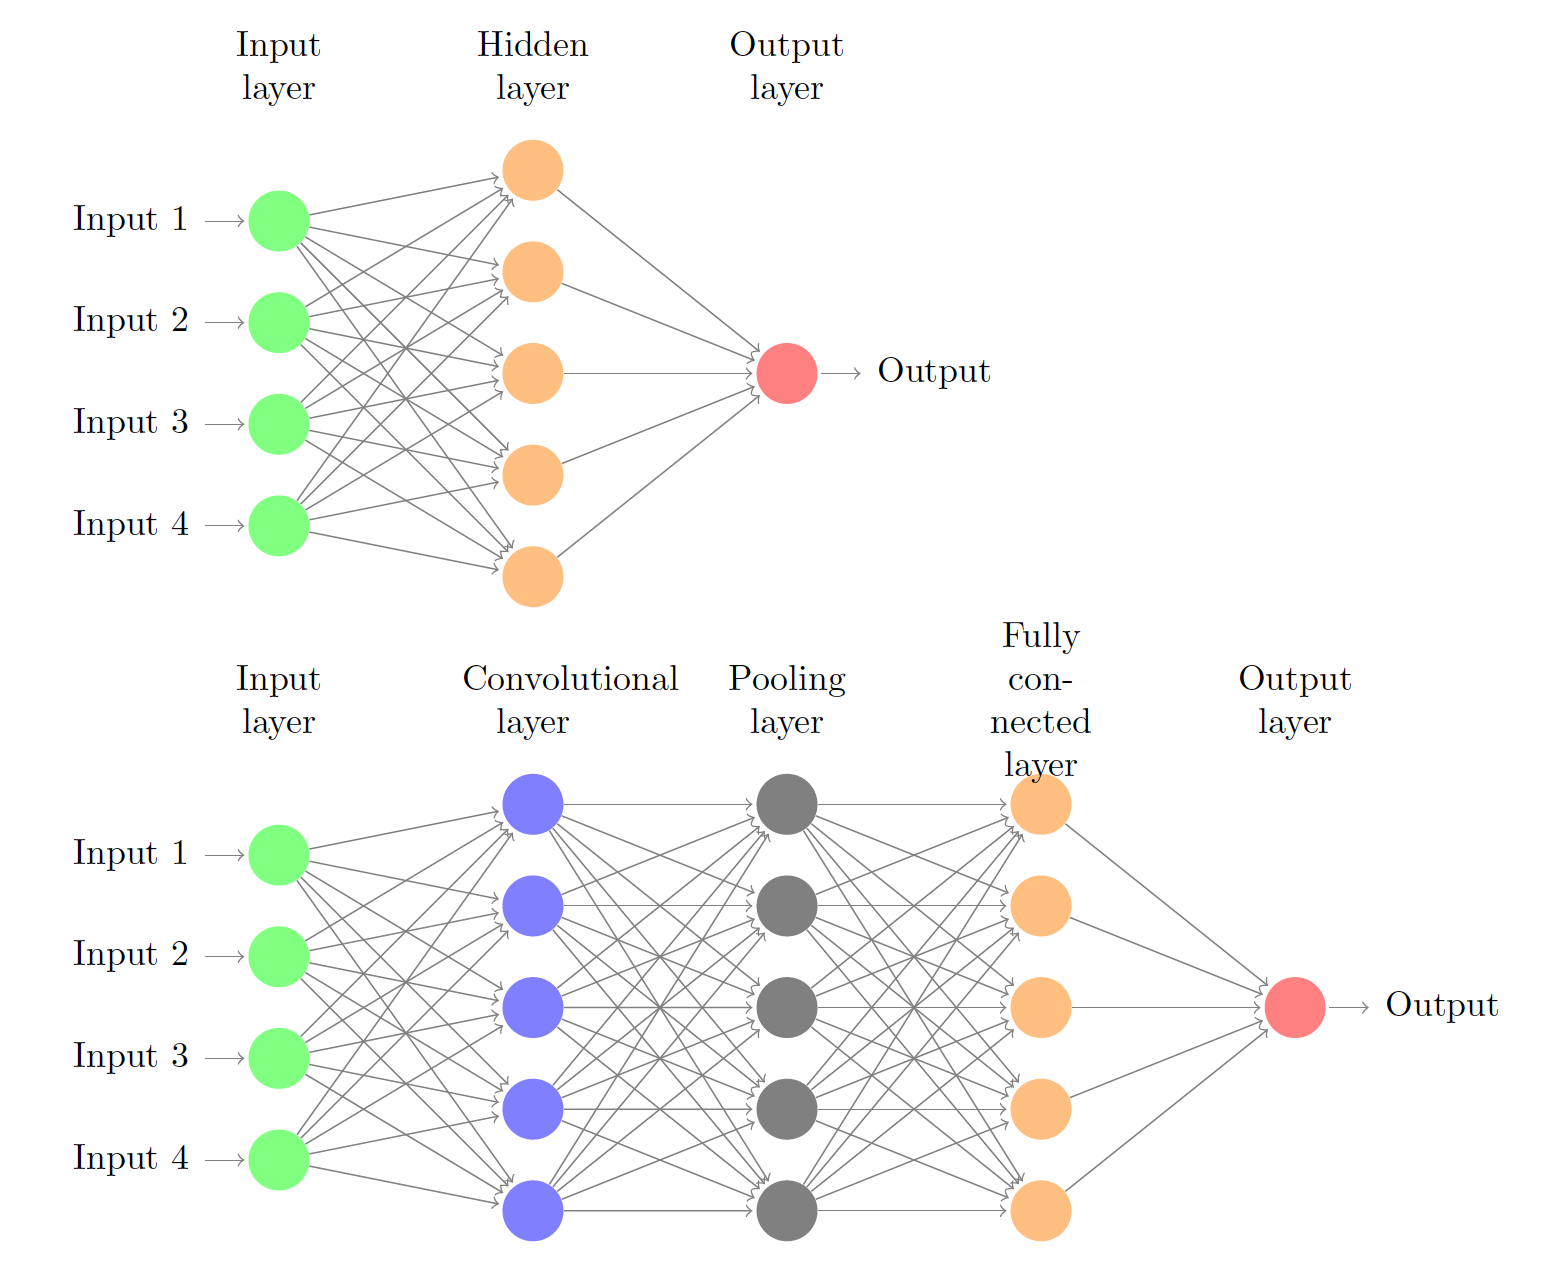
\includegraphics[scale=0.563]{figures/NN_arch.png}
\end{adjustbox}
\end{figure}


The key functionality of the CNN layers can be described in the following areas: 

\begin{itemize}

\item The input layer of CNN will work as same as the ANN input layer by distributing the input values to the next level of layer.
 

\item The next layer of the CNN is the `Convolutional layer'. This layer regulates the output of the neurons connected to the local area of the input. This process is done by the scalar product of the local input area and the weights. Each neuron of this layer takes input from the previous layers rectangular section. Therefore, convolutional layer is an image convolution of the previous layer. 

\item The down-sampling by the spatial dimensionality of the connected input area is then performed by the next layer which is the `Pooling layer'. This layer takes a small block from the convolutional layer and produces a single output by subsampling. Therefore, this layer reduces the number of bounds are placed in that activation. 

\item `Fully connected layer' performs just like it works on a traditional artificial neural network. This layer produces the class scores of the activations. This scores are then used for doing different types of classifications. Also in order to improve overall performance ReLU (rectified linear units) can also be used between these layers. 



\end{itemize}

More mathematical operations about CNN are discussed in the later part of the thesis. 

\begin{figure}
\centering
\begin{adjustbox}{addcode={\begin{minipage}{\width}}
{\caption{A sample Convolutional neural network architecture~\cite{convolutionalneuralnetworks} } 
\label{cnn}
\end{minipage}}}
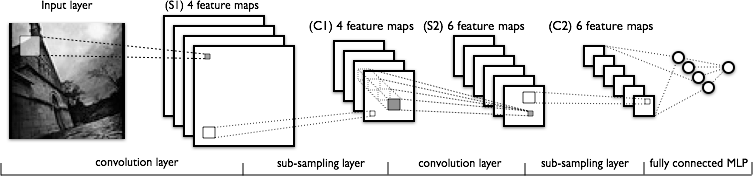
\includegraphics[scale=0.7]{figures/CNNarch.png}
\end{adjustbox}
\end{figure}






\subsection{Big Data \& its Challenges}
\label{int:Challenges} 
In order to state a huge amount of data which can not be handled by the traditional data management methods because of the size and the complexity of the data, the term ``Big Data" was first introduced by Roger Magoulas from O’Reilly media in 2005. According to Sam Madden an associate professor of MIT, Big Data is ``data that's too big, too fast, or too hard for existing tools to process."  

%[[[[ADD big data DEFINIIONS FROM Forecasting with Big Data: A Review]]]]


To overcome this Big Data and extracting information from it we should discuss the 5 V's of the Big Data. These 5 V's includes describing the size of the data (Volume) of different categories (Variety) below the manageable rate (Velocity) and the authenticity (Veracity) as well as the importance of the data(Value) [figure~\ref{5v}].



\begin{figure}
\centering
\begin{adjustbox}{addcode={\begin{minipage}{\width}}
{\caption{5 V's of Big Data } 
\label{5v}
\end{minipage}}}
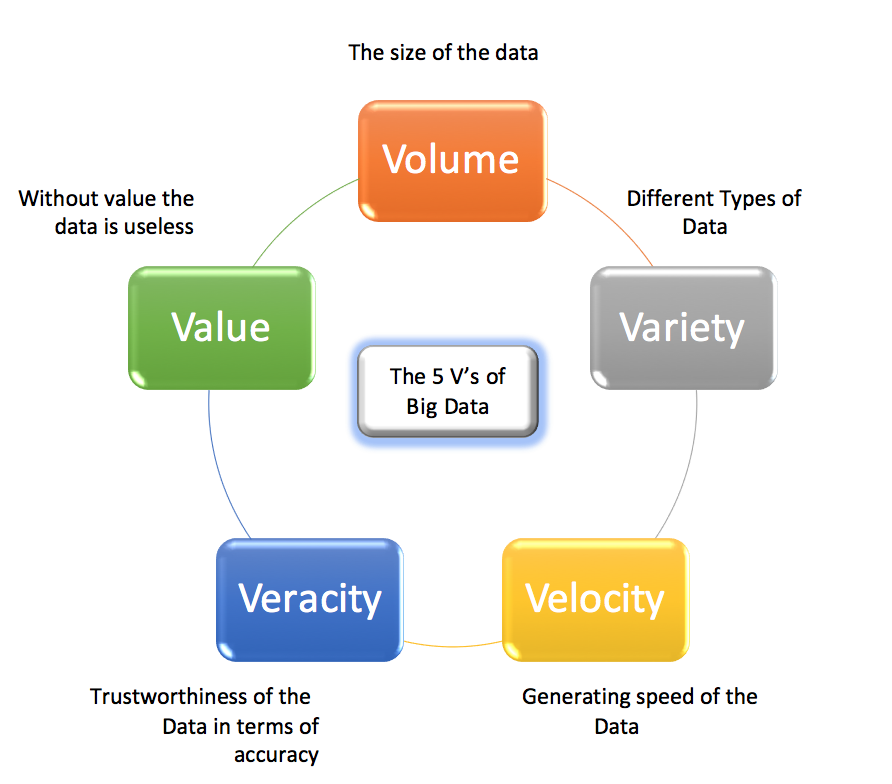
\includegraphics[scale=0.7]{figures/5_vs_safat.png}
\end{adjustbox}
\end{figure}

In order to forecast future,  some important challenges often develops from the nature of the data. Few of them are listed below.


\begin{enumerate} 
\item Statistical impact:  Without getting mislead by randomness, it is important to get precise and significant statistical results. 
\item Analytics construction: There is no fixed rule or way to decide the optimal architecture of the analytic system. 
\item Disseminated mining: To have distributed versions of the methods used, it is must to carryout a lot of research work and theoretical and practical analysis. 
\item Data compression: Storing big data efficiently is also a very important challenge when it comes to Big Data. We can either store the important parts of the data or we can sample the data in a way where we think data is more relevant.
\item Time changing data: Sometimes data changes a lot over the time, for this thesis the data changes significantly over the time. Therefore, it is important for used methods to adapt over the time.
\item Visualization: Another important challenge with dealing with big data is to analyze how to visualize the data to find/solve the problem. 
\end{enumerate}

By overcoming these challenges my goal was to forecast the bike share usage of New York City as well as to find different ways to improve this bike share service. In my thesis, I have considered a set of bike share usage data as image processing problem and in the following part of my thesis I will discuss more about my method and why I chose this approach.



\section{Thesis Outline}
\label{outline}

This thesis is structured in the following sections :

Chapter 2, begins with a review of demand forecasting with Big Data and the problems and potentials are presented, as well as some challenges and applications. This chapter also provides some reviews on the approached topic of bike share service demand forecasting.  
Chapter 3, explains the problem of bike share service and then presents the details about the dataset which was used to build the forecasting model. Furthermore, a few preliminary analysis of the data as well as the methodology of the proposed model is described.    
Chapter 4, presents the feature selection process of the data and brief explanations of the baseline models and evaluation metrics followed by the results and discussions of the proposed model. 
Chapter 5, summarizes the contribution of the thesis as well as some future works are mentioned. 








%%%%%%%%%%%%%%%%%%%%%%%%%%%%%%%%%%%%%%%%%%%%%%%%%%%
%
%  New template code for TAMU Theses and Dissertations starting Fall 2012.  
%  For more info about this template or the 
%  TAMU LaTeX User's Group, see http://www.howdy.me/.
%
%  Author: Wendy Lynn Turner 
%	 Version 1.0 
%  Last updated 8/5/2012
%
%%%%%%%%%%%%%%%%%%%%%%%%%%%%%%%%%%%%%%%%%%%%%%%%%%%
%%%%%%%%%%%%%%%%%%%%%%%%%%%%%%%%%%%%%%%%%%%%%%%%%%%%%%%%%%%%%%%%%%%%%%
%%                           SECTION III
%%%%%%%%%%%%%%%%%%%%%%%%%%%%%%%%%%%%%%%%%%%%%%%%%%%%%%%%%%%%%%%%%%%%%
%\setlength{\parindent}{2em}
%\setlength{\parskip}{1em}

\chapter{\uppercase{Literature Review}}

\section{ Theory}
\label{DST}
As previously mentioned, forecasting using Big Data is a ground-breaking sensation which is  one of the most discussed and one of the most important topic in the modern age. In this section a detailed review of the use of Big Data for forecasting with identifying the problem, potential \& challenges come with it also the related applications is presented. For obtaining meaningful forecasting results from Big Data is often faced with a lot of challenges such as- skills used, software and hardware, architecture of the algorithm, signal to noise ratio, statistical importance as well as the nature of the data itself. Even though all this challenges are continuously trying to impede the forecasting, many fields like Energy, Economics, Population dynamics are the main exploiters of it. With some common tools like Bayesian, Regression, Neural Network models are implemented for these type of forecasting with the availability of Big Data. 


\subsection{The Basics}
\label{Basics}

The arrival of Big Data is becoming history now as industries around the world are generating enormous amounts of data every second. Therefore it is very important for organizations to respond to this digital growth of asset and adopt necessary tools to exploit it for their own benefit. As~\cite{varian} states that there is a need for adoption of data mining techniques which can support in modelling the complicated connections of the characteristics present in Big Data. Also in current years, organization felt the importance of the risk management due to the recent financial crisis. According to~\cite{silva} corporations are now trying to minimize associated threats of maximizing their opportunity by using risk management tools. Hence, forecasting using Big Data has the potential and the ability to boost the organizational performance whereas empowering enhanced risk management~\cite{brown2011you}.
Conversely, Not every author is agreeing with the Big Data sensation. In~\cite{KAUFMAN199629} Poynter describes that Big Data will be more intuitive for connecting dots rather than painting a whole new picture. According to~\cite{walker} the year 2013 was the year to get familiarized with Big Data and 2014 is the year to start exploiting the Big Data for profitable gains. This chapter will provide a brief knowledge about Demand Forecasting in current time using real world Big Data also the challenges and applications of it. 


\section{``Potential"  and  ``Problem"}
\label{PaP}


Demand forecasting using Big data has a lot of different opportunities for lucrative gain. Companies have already started exploiting Big Data in order to forecast demand and work accordingly in order to improve better management and also increase revenues. Fashion companies like EDITD are trying to forecast future fashion trend demands by using the data collected from social media. Netflix used Big Data for decision making before starting their own TV show ‘House of Cards’ which then became very successful. Airline companies are also relies on the demand forecasting very much. Therefore, we can clearly see that the potential behind demand forecasting using Big Data are huge and actually overwhelming. But this is so astonishing that sometimes it becomes scary as in~\cite{duhigg2012companies} author described a story where a woman complained about a ‘Target’ store for sending her high school daughter pregnancy related coupons. But a few weeks later she apologized as her daughter was in fact pregnant~\cite{duhigg2012companies}. 


\section{Challenges}
\label{Challenges}

Demand forecasting using Big Data poses a lot of challenges which we must overcome in order get any meaningful outcomes from the data. It is also vital to know that Big Data's obtainability does not end the problems~\cite{ba}, therefore, in this section I will be primarily focusing on the challenges. Some of the challenges are associated with the techniques, assumptions~\cite{silver2012signal} while~\cite {west_2013} suggests that absence of theoretical support of Big Data is also a major concern. 


\subsection{Skills}
\label{Skills}

One of the major challenges while trying to forecast demand using Big Data is the expertise needed and the availability of experts in this specific tasks.~\cite {arribas2014accidental} shows that the importance of cutting-edge skills in order to deal with Big Data and~\cite{wesson2014big} states the shortage of the data scientists who are able to tackle this problem. Traditional researchers and scientists are working on old methods for decades and now this emerging era of Big Data is a challenge in itself. Therefore, inappropriateness of these traditional methods which were used on the old data types are hampering current world from forecasting using Big Data~\cite{skupin20081}~\cite{arribas2014accidental}. For more than 50 years these traditional statisticians are working on those outdated techniques, which makes it very difficult to develop new skills for Big Data forecasting~\cite{einav2014data}. Hence, it is necessary for current big educational organizations all over the world to modify their curriculum to adopt the need for new generations of statisticians by include the skills needed for understanding, analyzing and forecasting with Big Data. Thus we can make sure that in future we will have better skills to tackle this new very powerful asset of Big Data and also will be able to forecast more important insights from the data. 



\subsection{Unwanted Data / Noise}
\label{noise}

Unwanted data or noise is actually making it very difficult to forecast something accurately using Big Data. In~\cite{silver2012signal} the author points out at this problem saying an increasing noise to signal ration is present in the current Big Data. As the data gets larger and larger, exploiting this data is also getting more difficult. Before the era of Big Data, traditional methods used to work relatively well in those smaller sets of data set, but now the Big Data sets consists of a lot of unwanted data or wrong data which makes forecasting very complex. Therefore, New techniques and methods needs to be applied in order to filter out those noises and restructure the data in a way so that we can get the most out of it. There are few techniques already present like- singular spectrum analysis which tries to filter out the noises from a time series and reform the time series with much less noise, which is also proved in ~\cite{hassani2009forecasting} ~\cite{hassani2015forecasting}.

\subsection{Hardware and Software}
\label{Hardsoft}

Almost all of us who is involved with statistical analysis have faced the problem that programs crashes after doing few thousands to iteration. Like~\cite{arribas2014accidental} says existing software to do statistical analysis are not powerful enough to do Big Data forecasting where~\cite{needham2013disruptive} says supercomputers are needed. Capable software’s are also as important as hardware’s and nowadays a lot of forecasting techniques are developed and some of them can automatically forecast problems~\cite{hyndman2013forecasting}. But these programs are not as reliable when it comes to deal with Big Data. Therefore, to make a powerful forecasting software it needs the required computing capability and only then we can effectively deal with forecasting as the data is getting bigger and bigger. 

\subsection{Algorithm Architecture}
\label{Algo}

Current data mining methods are often used for smaller datasets and are unable to perform in a satisfactory manner. Also many time this technique can not deal with the data which are not present in their main memory so data movement between locations are often poses a big problem~\cite{jadhav2013big}. Parallel programming or lambda architecture mentioned in~\cite{marz2015big} are samples of current ongoing research happening on this topic.

\subsection{Statistical Importance}
\label{Statistics}

While doing demand forecasting or forecasting with Big Data, it is very easy to make incorrect findings. The amount and the randomness of the data and the noise available in it increases the chance of getting a misleading forecasting report. On top of that finding an appropriate technique has always been a very difficult job for big data. In~\cite{lohr2012age} author also talks about the threat of making false discoveries. 

Apart from all these the phrase Big Data itself is a very difficult challenge while doing demand forecasting, due to its in-built characteristics. Very complex and unstable structure of the data makes it tough for data scientists to get any forecasting which is free from poor out of sample outcome~\cite{einav2014data}. Also it is very difficult to chose the correct method and while using deep learning it is very difficult to chose the number of hidden layers it should have due to the shapelessness of the data as it is continuously changing in real time. 



\section{Applications of Demand Forecasting}
\label{Application}

In this segment, we introduce the present applications which uses demand forecasting by exploiting data mining techniques on Big Data. The main reasons behind doing demand forecasting are :


\begin{itemize}
\item Cost reduction
\item Agility in the market
\item Estimating the financial capability
\item Planning ahead to meet necessities
\item Improve accuracy
\item Visualization - Relationships between different factors


\end{itemize}


\subsection{Energy Demand Forecasting}
\label{Energy}

Smart meters and advanced technology in the field of energy are the reason behind the huge data sets that are available currently. These Big Data have opened the door towards endless opportunity for improvement in better energy management and conservation system as well as new energy systems. A lot of experiments have been carried out in the field of energy like, in~\cite{nguyen2010short} Nguyen and Nabney tried to exploit the Big Data from the British Energy organizations and they used few different models to evaluate the wavelet transform like, linear regression, GARCH, MLP and Radial basis functions. They found that MLP or GARCH with wavelet transform are the best models for forecasting electricity demands as well as the gas price. 


\subsection{Health Care Demand Forecasting}
\label{Health}

By using the Big Data in health care field it is possible to improve charge capture and also can reduce the denial rate of reimbursement. According to~\cite{callahan2004effective} it is also possible to do location based forecasting in order to coordinate surgeon preference information and also forecasting demand based on the patient demographics, clinic scheduling as well as seasonal demands. These results provide lower cost for the preparations of cases, reduces inventory levels in OR, supports clinics for much better planning and budgeting to introduce new or to expand current surgical agendas also improving the service and fill rates which leads those clinics to improve patient satisfaction, improved rating and productivity as well as patient safety. 

%\subsection{Tourism Demand Forecasting}
%\label{Tourism}

\subsection{Transportation Demand Forecasting}
\label{Transportation}
Demand forecasting in transportation is the method to predict the the number of people or the transportation mediums will be used in the future. This forecasting methods can then be applied on a range of different situations from forecasting traffic volumes on a particular road on a given day to forecasting passenger counts on trains or to forecasting number of ships will be there in a port. The reason behind these forecast is to predict what will be the demand in the future might be and also to specify the standard for planning and design to the most efficient transportation system. Application of demand forecasting in transportation allows us to improve overall transportation system, planning ahead to meet the requirements, developing the infrastructure capacity and design estimation. These can then make sure the approximation of the financial capability of the system as well as the environmental effects it has on them.   




In this thesis, I have used the Bike sharing system data of the New York city in order to forecast the demand of bike sharing service and to find ways to improve the service so that clients can get better experience from it. 

\section {Transportation Demand Forecasting : Bike Share Service Approach}

Forecasting ride sharing system usage is becoming very popular with the growing of industries like Uber-lyft. But substantial traffic in busy cities and aspiration of an environmental friendly way of transportation made bike share system very popular and attractive in recent years. Thus Bike share systems provide users an alternate and ecological way of conveyance by dodging personal car usage or taxis and staying stuck at traffic for a long period of time. This growing demand of bike sharing system making big cities to open their own bike share service for which currently more than 600 cities all over the world has the bike share program, allowing their residents to go from one place to another by renting bikes. Jensen et al.~\cite{jensen2010characterizing} also showed (in his case for Lyon) that sometimes it is faster than using personal car to go to places. Except the expenditure almost all the bike sharing program shares the similar technologies and it will be really exciting to predict the future usage of this amazing program and thus allowing users to plan their everyday trip more accurately with satisfaction. 

In May 2013, Citibank started a bike sharing service in New York City which is called City Bike. This is the nations leading bike share service with more than 10,000 bikes with 600 stations across the city where customers can rent a bike from any of those station for a quick, fun and reasonable ride on an as-needed basis. Users can obtain membership to rent the bikes and return the bike in an automated process via a network of stations throughout the city. City Bike share recently hit 10 million trips in a year and thus the system generates a lot of data which is very eye-catching field for researchers as it explicitly contains data about the departure station locations, age group and gender of the users, duration, arrival location and so on. Therefore, this service works like sensor network and can be used to study the movement flexibility in a particular city.  


Researchers around the world did some related research on the bike sharing system where they all tried to predict that a user can find a bike whenever he goes to the station. 



\subsection{Related Works}
\label {related}

Bike sharing system first started in Amsterdam in 1965 with the 1st generation `White bikes' and since then the popularity is increasing all over the world~\cite{demaio2009bike}.  Due to technological advancement the 3rd generation bike sharing system is available now, where it is possible to do bicycle reservations, information tracking, automated pickup and dropoff system~\cite{shaheen2010bikesharing}. This IT based integrated system for bike share programs made it possible to collect its data to do research and find possible ways to improve the system. 

Researchers around the world did some related research on the bike sharing system and these are mainly focused into four different problems. Strategic program scheme, quality improvement, demand analysis and rebalancing issue.
Almost all the major cities around the world already planned or is planning or considering execution of this bike share system. For the first problem, estimating potential demand in order to optimize location, deel’ollio et al.~\cite{moura2011implementing} presented an inclusive approach for implementation. Location is also another issue which was widely discussed in Martinez et al.~\cite{martinez2012optimisation} and Prem Kumar et al.~\cite{kumar2012optimizing} where they propose MIP models to tackle this issue. Also a trade off model for the interest of both customers and sponsors were proposed in~\cite{lin2011strategic}.

There has been also several research focusing on the second problem which is the quality improvement. Raviv et al.~\cite{raviv2013static} proposes a model for probable user’s displeasure in every station based on a queuing system with finite capacity. Nair et al.~\cite{nair2013large} and Nair and Miller~\cite{miller2010fleet} decompose system-wide reliability into a set of dual-bounded chance constraints for every station. By assumption of waiting customers~\cite{leurent2012modelling} shows bike sharing stations as a dual Markovian waiting system. 
 
Similar to this thesis there has been few research about Demand analysis where the analysis is mainly divided into two sections – 1) forecasting future demand, 2) understanding factors for administrative decisions. Kaltenbrunner~\cite{kaltenbrunner2010urban} tries to predict the system inventory state also suggests making this information available to users. Rixey et al.~\cite{rixey2013station} investigates the effects of demographic and built environment characteristics near three bike sharing stations on bike sharing ridership levels in three operational U.S. systems. The regression analysis identifies a number of variables as having statistically significant correlations with station-level bike sharing ridership and identify station locations that will serve the greatest number of riders. Borgnat and Abry~\cite{borgnat2011shared} , Froehlich and Oliver~\cite{froehlich2008measuring}, Lathia et al.~\cite{lathia2012measuring} and Borgnat et al.~\cite{borgnat2009studying} identify a temporal demand pattern and forecast the number of rentals. Giot and cherrier~\cite{giot2014predicting} attempts to predict the bike share usage up to one day ahead with an hour of granularity and compared how adaboost regressor, ridge regression, SVR, random forest nad gradient boosting regressor performs on dataset on two years. Their results sows that most regressors are sensitive to over-fitting. 

For the fourth problem, Shu et al.~\cite{shu2010bicycle} showed that estimate rebalancing operations can lead to an additional 15-20\% of trips supported system-wide. Chemla et al.~\cite{chemla2013bike} present a branch-and-cut algorithm for the single-vehicle problem, with results on instances of up to 100 stations. Lin and Chou~\cite{lin2012geo}, rather than simply using Euclidean distance they proposed an optimization way taking road conditions, traffic regulations, and geographical factors into account. Their actual distance path calculation is used to implement a exploratory for the VRP. Naturally, using actual distances would lead to decreased costs in practice. Yoon et al.~\cite{yoon2012cityride} proposes auto regressive moving average model to help bike share users to navigate around the city. By giving the starting and end point the application can suggest which stations would be best to use by considering the walking time and biking time and available return slots at the end station. This model is useful for stationary signals and the bike share system which is varying over time.  

From the researches mentioned above it can be observed that there are many research going on in different topics related to bike share system but for the forecasting bike usage people are mainly using machine learning models with space and time series features and building applications to help customers navigate around the city easily. 
For this thesis, I present a Convolutional Neural Network based demand forecasting model where the bike usage data is treated as images and solved a regression problem using CNN. Results also shows the efficiency of the model. 




%%%%%%%%%%%%%%%%%%%%%%%%%%%%%%%%%%%%%%%%%%%%%%%%%%
%
%  New template code for TAMU Theses and Dissertations starting Fall 2012.  
%  For more info about this template or the 
%  TAMU LaTeX User's Group, see http://www.howdy.me/.
%
%  Author: Wendy Lynn Turner 
%	 Version 1.0 
%  Last updated 8/5/2012
%
%%%%%%%%%%%%%%%%%%%%%%%%%%%%%%%%%%%%%%%%%%%%%%%%%%%
%%%%%%%%%%%%%%%%%%%%%%%%%%%%%%%%%%%%%%%%%%%%%%%%%%%%%%%%%%%%%%%%%%%%%%
%%                           SECTION IV
%%%%%%%%%%%%%%%%%%%%%%%%%%%%%%%%%%%%%%%%%%%%%%%%%%%%%%%%%%%%%%%%%%%%%


\chapter{\uppercase{Methodology}}



\section {The Problem}
Like any other program this bike sharing service also suffers few major problems. Bike rebalancing problem being the most important and significant of them all. This rebalancing problem occurs when a bike station is either full or empty and makes it difficult for users to rent or to park their rented bike. Thanks to the current prediction systems, it is possible to predict the usage of the bike share program and therefore allowing the users to have better experience of the bike share system. The objective is to make sure the users can walk to a bike docking station and find bikes to rent and also to discharge the rented bikes without having to wait for another user or going to another station to do that.

In order to find the problem and to set the goal of my thesis, first I did some statistical analysis on the bike share data and from those studies I saw that the distribution of the data is not balanced and same goes for gender distribution of the subscribers. Therefore, I tried to find a solution to overcome this two problem which is to forecast hourly rental bike demand for both men and women. I treated this problem as a regression forecasting with time series features and proposed Convolutional Neural Network (CNN) to do the forecasting which outperforms other traditional machine learning methods. I have used the data obtained from the City Bike system and weather data to forecast hourly rental demand of the Bike share system. 

\section{Datasets}

The goal of this thesis is to forecast bike demand using the users historical bike usage patterns along with the weather data and user's information in a time series arrangement. Therefore, this thesis attempts to answer the following questions : ``How many bikes are needed every hour?", ``Who are renting those bikes?", ``How weather is affecting the bike share usage?", ``Is it a holiday, weekend or normal weekday?". Therefore, datasets should contain three major information: 1) bike renting time and details, 2) users information, 3) weather data as well as 4) holiday/weekday-weekend information.

Collected dataset on the city bike share system contains details about the trip and the user who is renting it from January 2015 to July 2015. I have also collected weather datasets during that period and used January 2015 to June 2015 data sets to create the training set and the rest for testing set. 

Figure~\ref{datasets} shows the overview of the dataset preparation to build the forecasting model. Detailed information about the dataset extracting and processing will be discussed later in this chapter. 



\begin{figure}
\centering
\begin{adjustbox}{addcode={\begin{minipage}{\width}}
{\caption{Dataset Overview.}
\label{datasets}
\end{minipage}}}
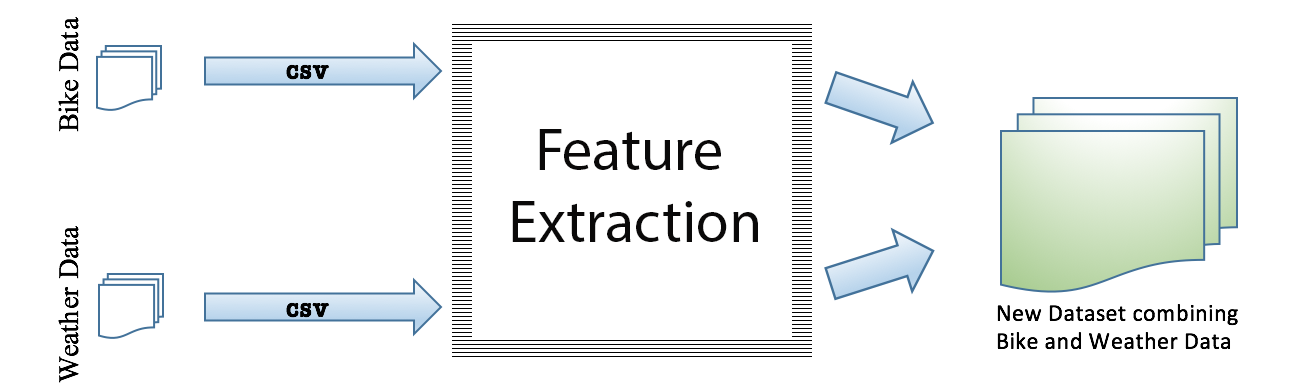
\includegraphics[scale=0.7]{figures/Dataset_overview.png}
\end{adjustbox}
\end{figure}


\subsection {New York City Bike Dataset}
\label{NYCdata}

The city bike system website provides historical datasets for all the researcher interested to carry out their research. This dataset is in CSV - comma separated values format. This dataset contains 6 key variables which are key to this thesis - `tripduration', `starttime', `stoptime', `usertype', `birthyear', `gender'.  This deals with the first two major topics which mentioned are above – 1) Bike renting time and details, 2) Users information. 

\begin{table}
\centering
\caption{Details of the Citi Bike Trip data }
\label{bikedata}
\vspace{1ex}
\begin{tabular}{||c||c |p{6.5cm} |c||}\hline
Field name & Type  &  Explanation & Information  \\\hline\hline
tripduration & Numeric & Duration of the ride in seconds & 1 \\\hline
starttime& Date& Start date and time of the trip  & 1 \\\hline
stoptime&Date &Stop date and time of the trip & 1 \\\hline
start station id&Numeric & Starting station id & 1 \\\hline
start station name& Character& Starting station name& 1 \\\hline
start station lattitude& Numeric& Starting station latitude& 1 \\\hline
start station longitude&Numeric &Starting station longitude & 1 \\\hline
end station id&Numeric &End station id & 1 \\\hline
end station name&Character &End station name & 1 \\\hline
end station lattitude&Numeric &End station latitude & 1 \\\hline
end station longitude&Numeric &End station longitude & 1 \\\hline
bikeid& Numeric& Bike identification& 1 \\\hline
usertype& Character& Type of user (Subscriber = Annual member, Customer = 24 hr/ 7 day pass) & 2 \\\hline
birthyear&Date &Users birth year & 2 \\\hline
gender& Numeric& Gender of the user (0=unknown, 1= male, 2= female)& 2\\\hline
\end{tabular}
\end{table}


The City Bike dataset has 3,379,904 entries of bike rental data and it all has the content showed in table~\ref{bikedata}.  Target bike rental dataset is then designed to get the time information, which is found by splitting the `starttime' into `hour', `month', `day'. Total number of rented bikes per hour can be then grouped in one field. Table~\ref{target_bikedata} shows the extracted details from those bike datasets which is then used for the experiment. 


\begin{table}[]
\centering
\caption{Target dataset of the Citi Bike trip data}
\label{target_bikedata}
\begin{tabular}{||l||l|l|l||}
\hline
Source                    & Name         & Type             & Information                            \\\hline\hline
\multirow{4}{*}{startime} & hourly count & numeric          & Total number of rented bike per hour   \\ \cline{2-4} 
                          & hour         & numeric          & Hour data                              \\ \cline{2-4} 
                          & day          & numeric          & Day                                    \\ \cline{2-4} 
                          & month        & numeric          & Month                                  \\ \hline
\multirow{2}{*}{usertype} & subscriber    & binary & Subscriber count                       \\ \cline{2-4} 
                          & customer     & binary & Customer count                       \\ \hline
birthyear                 & age          & numeric          & Age of the user                        \\ \hline
\multirow{3}{*}{gender}   & unknown      & binary & Unknown gender information of the user \\ \cline{2-4} 
                          & male         & binary & Male count                             \\ \cline{2-4} 
                          & female       & binary & Female count                           \\ \hline
\end{tabular}
\end{table}


\subsection {New York City Weather Dataset}
\label{NYCweatherdata}

For this thesis I have collected some historical New York City weather data from the NOAA (National centers for environmental information) website. From this dataset 8 key factors were chosen. These are – Date (Year, Month, Day), snow depth, snow fall, average wind speed, trip, precipitation. The target dataset from the weather data is shown in Table~\ref{target_weatherdata}.

\begin{table}[]
\centering
\caption{Target weather dataset}
\label{target_weatherdata}
\begin{tabular}{||c||l|l||}
\hline
Name               & \multicolumn{1}{c|}{Type} & \multicolumn{1}{c||}{Information}                         \\ \hline\hline
Year               & numeric                   & Year count                                               \\ \hline
Month              & numeric                   & Month count                                              \\ \hline
Day                & numeric                   & Day count                                                \\ \hline
Snow depth         & numeric                   & Snow depth level (in)                                    \\ \hline
Snow fall          & numeric                   & Snow fall rate (in)                                      \\ \hline
Average wind speed & numeric                   & Wind speed (mi)                                          \\ \hline
Temperature       & numeric                   & Temperature (F)                                          \\ \hline
Precipitation      & numeric                   & Rain, snow, sleet, or hail that falls to the ground (in) \\ \hline
\end{tabular}
\end{table}



\subsection {New York City Holiday Dataset}
\label{NYCholidaydata}


I have also collected dataset of the holiday during the period of Jan'2015 to July'2015 shown in figure~\ref{Holiday} and used it to build the training set of my model. There were 8 national holidays during the time period of the datasets related to this experiment of the year 2015 in USA. With this holiday weekend and weekday binary values will also be included in order to create the target dataset which is shown in 
Table~\ref{target_holidaydata}.  


\begin{figure}
\centering
\begin{adjustbox}{addcode={\begin{minipage}{\width}}
{\caption{Holiday list of NYC in 2015 (Jan-July) ~\cite{holidaysinnewyork}}
\label{Holiday}
\end{minipage}}}
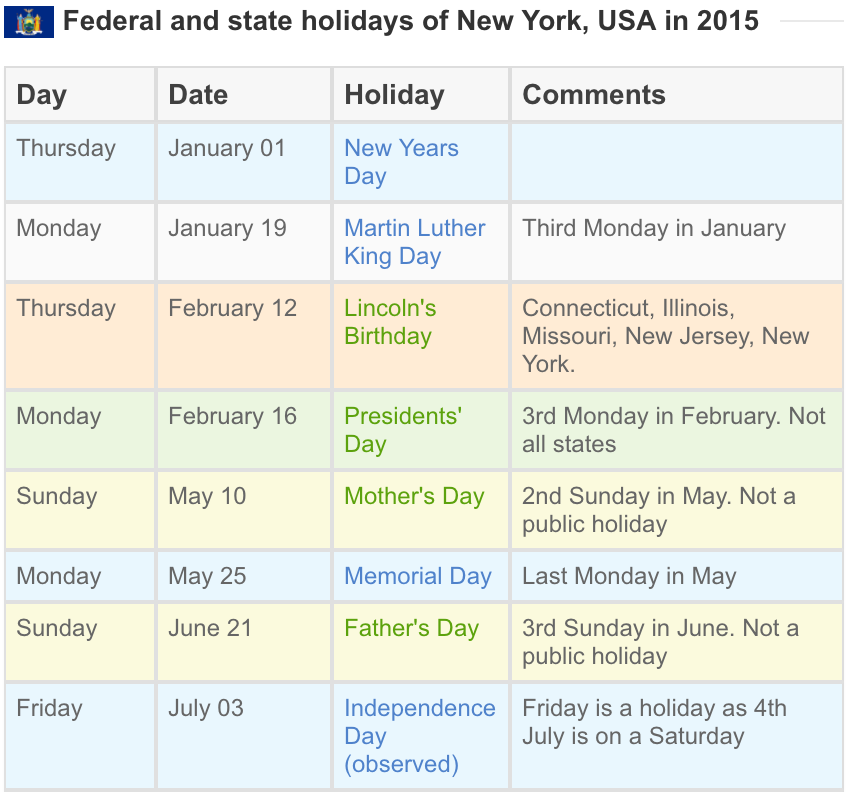
\includegraphics[scale=0.7]{figures/Holiday_nyc.png}
\end{adjustbox}
\end{figure}


\begin{table}[]
\centering
\caption{Target Holiday dataset}
\label{target_holidaydata}
\begin{tabular}{||c||l|l||}
\hline
Name                  & \multicolumn{1}{c|}{Type} & \multicolumn{1}{c||}{Information}           \\ \hline \hline
Holiday               & binary                    & Holiday binary value                       \\ \hline
Weekday               & binary                    & Weekday binary value                       \\ \hline
Weekend (not holiday) & binary                    & Weekend which are not holiday binary value \\ \hline
\end{tabular}
\end{table}



\section {Statistical Analysis}
\label{statistics}

In order to find the problem and to set the goal of my thesis, first I did some statistical analysis on the bike share data and from those studies I saw that the distribution of the data is not balanced and same for the distribution of the gender of the subscribers. Therefore, I tried to find a solution to overcome this two problem which is to forecast hourly rental bike demand for both men and women. I treated this problem as a regression forecasting with time series features and proposed Convolutional Neural Network (CNN) to do the forecasting which outperforms other traditional machine learning methods. I have used the data obtained from the City Bike system and weather data to forecast hourly rental demand of the Bike share system.


Getting more insights and understanding of the data before applying any machine learning tools is very important when it comes to forecasting. First we saw that there are two types of users in those data - subscribers and customers. So, then I tried to plot the trend of the bike share rentals between them. 


\begin{figure}
\centering
\begin{adjustbox}{addcode={\begin{minipage}{\width}}
{\caption{Customer vs Subscribers rental trend }
\label{custVSsubs}
\end{minipage}}}
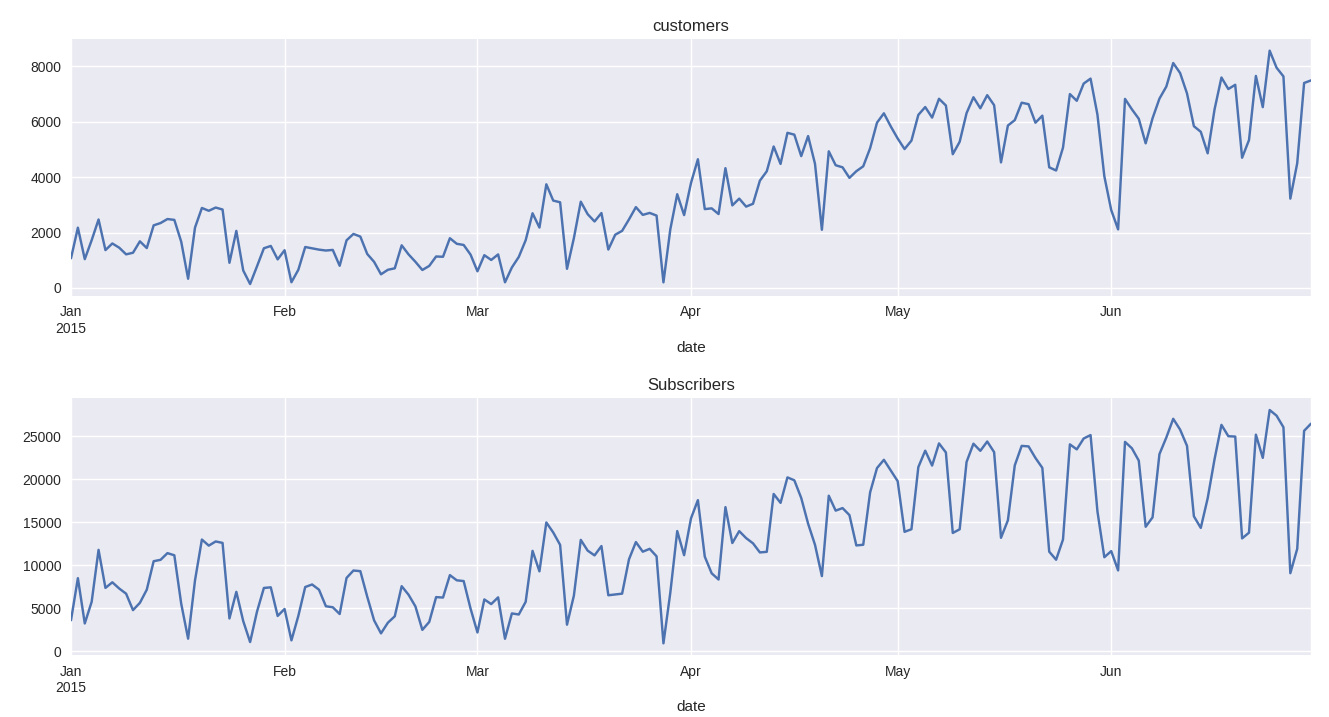
\includegraphics[ height=9cm, width=15cm]{figures/analysis/month.png}
\end{adjustbox}
\end{figure}

From this figure~\ref{custVSsubs} we can see that the customer count is almost less than $1/3$ in count and the distribution of the data is unbalanced which can be because of a lot factors like weekend, weekdays, good or bad weather, holiday etc. 


\subsection {Weekly Distribution}
\label{week}

To get more deep into this unbalanced distribution of the data, more deep analysis of the data is needed. Rather than getting the rental demand trend in monthly basis, weekly distribution is then applied. This time the weekly data is divided in gender basis, which is another important factor for this thesis. figure~\ref{maleVSfemale} shows the weekly average demand trend and from this figure we can see that rental demand significantly decreases when the weekend comes. This figure also shows a very valuable comparison between ``male" and ``female" rental demands. Females are $1/4$ less likely to rent a bike than males in New York City. There are also some unknown data which are the users who did not provide their gender details. The unknown data was really low during the weekdays but in the weekends the count rises high enough to even surpass female counts. Which also tells us that during weekends alot of people who are not subscribers, likes to roam around in the city using this bike sharing system. 

Doing daily analysis it was also found that the average number of bike rental demand per day for male is about $13$ thousands where for female it was $3,602$ and for unknown data it was around $2$ thousands. Another gender distribution is also shown in the figure~\ref{genderpie} where $69.3\%$ of rental data is provided by male and only $19.3\%$ of them are female, rest $11.4\%$ being the unknown categories. 
    


\begin{figure}
\centering
\begin{adjustbox}{addcode={\begin{minipage}{\width}}
{\caption{Male vs Female average rental demand per week}  
\label{maleVSfemale}
\end{minipage}}}
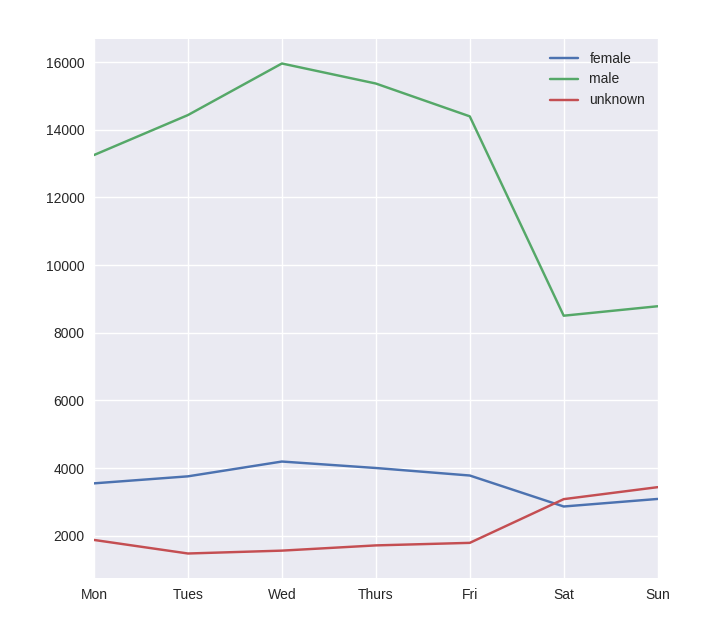
\includegraphics[scale=0.7]{figures/analysis/day.png}
\end{adjustbox}
\end{figure}



\begin{figure}
\centering
\begin{adjustbox}{addcode={\begin{minipage}{\width}}
{\caption{Gender distribution in rental demand of bikes}  
\label{genderpie}
\end{minipage}}}
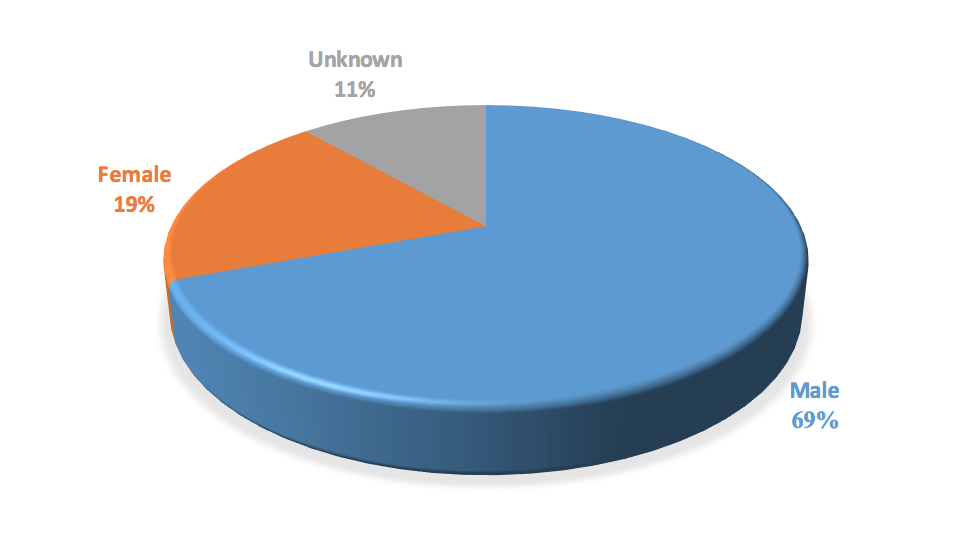
\includegraphics[scale=0.8]{figures/analysis/genderpie.png}
\end{adjustbox}
\end{figure}




\subsection {Trip Duration Frequency}
\label{trip}




A detailed analysis on the trip duration is also carried out in order to understand user behaviors behind renting bikes from this bike sharing system. There is also an extra charge after $30$ minutes of use of bike in one go for customers and after $45$ minutes for subscribers as shown in figure~\ref{duration} . So therefore, users are more likely to avoid this extra charge as one of the main reason behind using bike share system is to move around the city in an affordable way. But, from the data we observed an interesting tendency of the users. The maximum duration being $97744.35$ minutes which is either lost and then found or just an outlier in the data which we can neglect and minimum duration found is a minute. The mean duration is around $12.5$ minutes and most importantly more than $75\%$ is around $14$ minutes. So, from this we can realize that people mostly uses bike share program for short trips in the city.

\begin{figure}
\centering
\begin{adjustbox}{addcode={\begin{minipage}{\width}}
{\caption{Trip duration distribution between subscribers and customers} 
\label{duration}
\end{minipage}}}
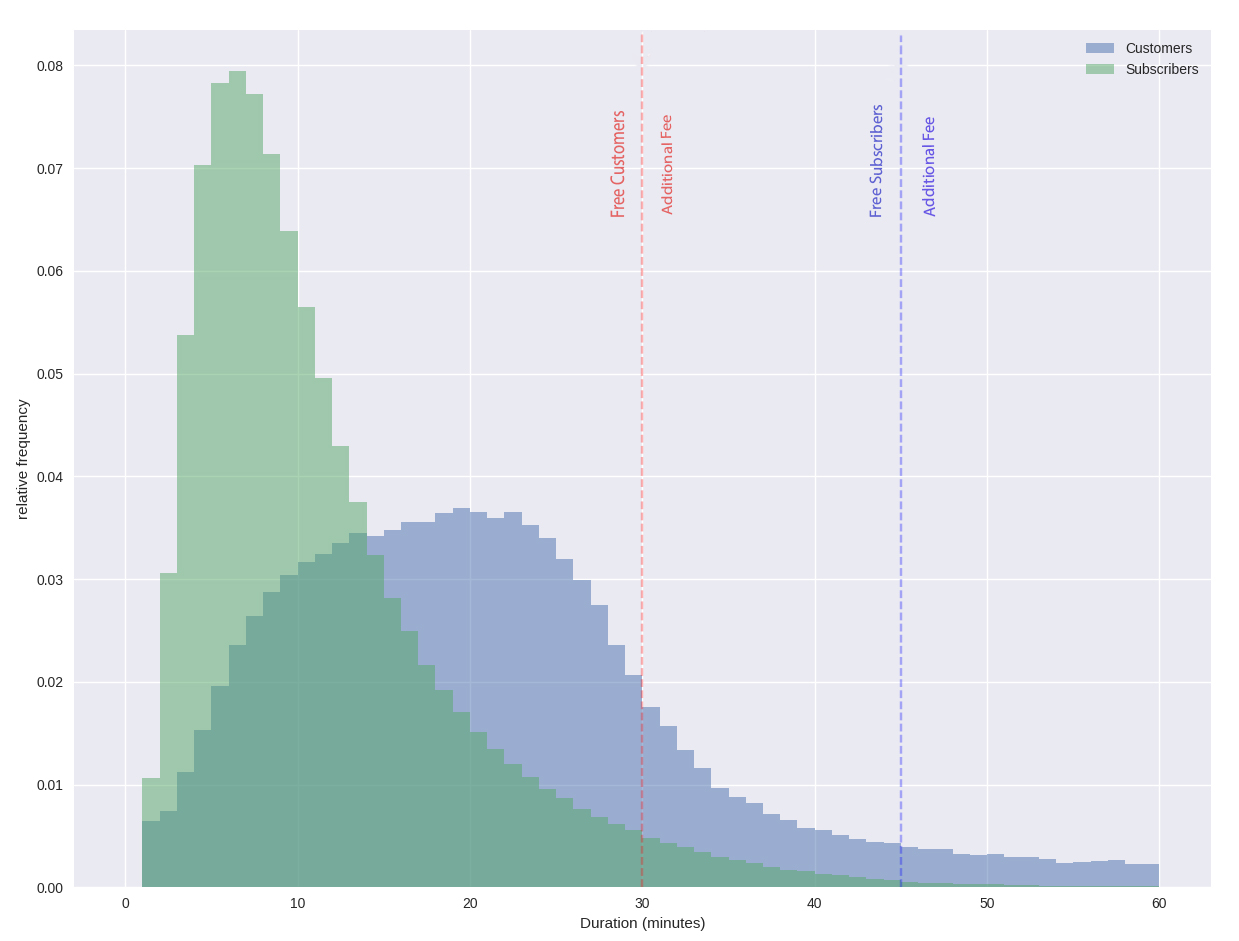
\includegraphics[width=1.0 \textwidth]{figures/analysis/duration.png}
\end{adjustbox}
\end{figure}

\subsection {Hourly Distribution}
\label{hourly}


Comparing the plots of the figure~\ref{hourly1} and figure~\ref{hourly2}, the shown graphs are based on the details about customers and subscribers and it shows that the pattern of the plot is noticeably different. ``Subscribers" who holds the annual pass for the bike share system displays `working' pattern. Which means the bike rental demand during the start and the end of the working hours are huge. Most people rents bike around 8:00 am and from 4:30 to 5:30 pm. ``Customers" who uses day or weekly passes shows random distribution of the data. It is also found that the maximum hourly demand of bikes in NYC in those time period is 3034 bikes and averages in about 540 bikes per hour, minimum being 1 bike.   

It is also found that the maximum age of a renter is a male being 77 years old and minimum is a female of 17 years old. The reason behind the minimum year is 17 is maybe because people under 17 do not hold credit cards. It is also very pleasing to see the mean values of age in general is 39 years. 



\begin{figure}
\centering
\begin{adjustbox}{addcode={\begin{minipage}{\width}}
{\caption{Hourly average rental demand in the City Bike trip data (Monday-Friday of Jan-June'2015)}  
\label{hourly1}
\end{minipage}}}
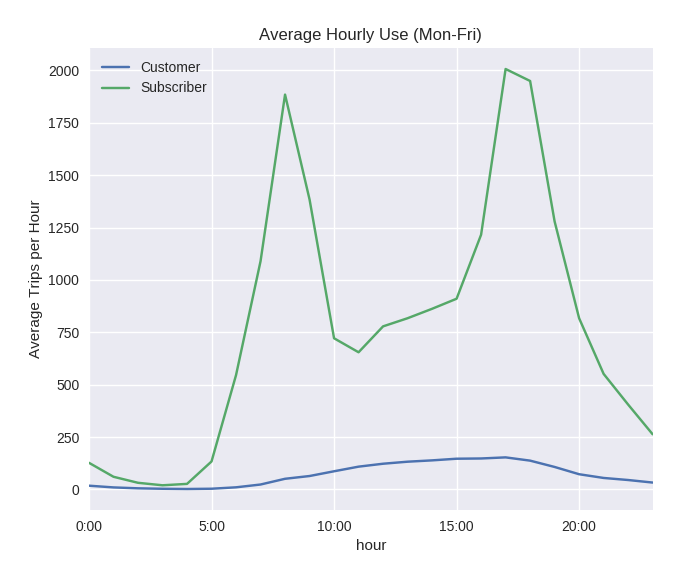
\includegraphics[scale=0.6]{figures/analysis/hourly1.png}
\end{adjustbox}
\end{figure}



\begin{figure}
\centering
\begin{adjustbox}{addcode={\begin{minipage}{\width}}
{\caption{Hourly average rental demand in the City Bike trip data (Saturday-Sunday of Jan-June'2015)}  
\label{hourly2}
\end{minipage}}}
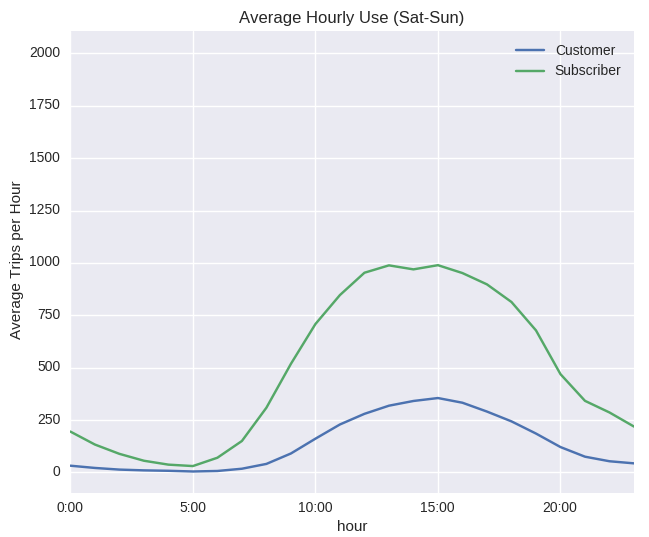
\includegraphics[scale=0.6]{figures/analysis/hourly2.png}
\end{adjustbox}
\end{figure}

After all this analysis of the data we can then conclude as the problem, where in these short bike trips between places it is very important to make sure users can rent and return a bike whenever they want. Therefore, the attempt of forecasting bike rental demand can play a vital role in order to predict the demand before it happens and thus rebalancing the whole system efficiently. Data also showed that customers normally uses bikes for short trips. So failing to deliver a rentable bike or a parking place in a desired station can cause the system to fail as a whole, as customers can sometimes just walk to the destination. Hence, it is very vital for a bike sharing program to make sure customers can get the best possible experience from it and stay subscribed. 


\section {Methodology}
\label{methodology}


Statistical results on the bike data prove that the distribution of the data is sometimes similar and therefore there is a big chance for researchers to find ways to improve the system. From the figure~\ref{maleVSfemale}, it shows the huge difference in rental demand count between male and female users in NYC. Therefore, there is big potential to increase the number of female users into this bike share system. In order to solve this matter, different bikes for different genders can be a very good option. By making the female bikes more appealing and colorful and also to design the bike to support female's body structure can provide better experiences for female users. 

This leads our main problem into two different problems. Forecasting and then providing enough bikes for both male and female users at any given hour. And the amount of female bikes needed can then also be determined from the rental demands of the female users. By doing this we can then forecast the adequate number of bikes needed also that every hour there will be enough bikes available for the users precisely.

\subsection{Convolutional Neural Network}
\label{CNNexpl}

Before discussing the problem and a way to solve it, it is necessary to understand how the Convolutional neural network works. As mentioned earlier in chapter 1 a CNN has three types of layers and the layer in use will decide the forward or back propagation is needed. A deep explanation of Forward and Back propagation of Convolutional layer and pooling layers are discussed below. 


\subsubsection{Forward Propagation}

Here it shows the computation of the layers in case of forward propagation :



\textbf {Convolutional Layers}:
To explain this section suppose we have $N \times N$ neuron layer trailed by the Convolutional layer. Then, the convolutional layer output $w$ will be $(N - m +1) \times (N - m + 1)$ if we use $m \times m$ filter. 

So, the pre-nonlinearity input to some unit $X_{ij}^{l}$  in the layer,  

$x_{ij}^{l}\sum_{a=0}^{m-1}\sum_{b=0}^{m-1}w_{ab}y_{(i+a)(j+b)}^{l-1}$ , this is done by summing up the weights by the filter sections from the earlier layer cells. After that the convolutional layer adds its non linearity – 
$y_{ij}^{l} = \sigma x_{ij}^{l}$.

\textbf {Max - Pooling Layers}: 
Max pooling layers basically takes some $k\times  k$ region and outputs the maximum single value for that region. For example, if they are getting input from a $N \times N$ layer then they will output a $ \frac{N}{k} \times \frac{N}{k}$ layer and using max function each $k \times  k$ block reduced to just a single value.

\subsubsection{Back Propagation}
The computation of the layers for back propagation :

\textbf {Convolutional Layers:}
Suppose the error function E and the error values at the convolutional layer is known. The error we know and the the calculation needed for the previous layer, with respect to each neuron output is the partial of E with respect to each neuron output$(\frac{\partial E}{\partial y_{ij}^l})$. By applying chain rule we can also compute the gradient. 

$\frac{\partial E}{\partial w_{ab}} = \sum_{i=0}^{N-m} \sum_{j=0}^{N-m} \frac{\partial E}{\partial x_{ij}^l} \frac{\partial x_{ij}^l}{\partial w_{ab}} = \sum_{i=0}^{N-m} \sum_{j=0}^{N-m} \frac{\partial E}{\partial x_{ij}^l} y_{(i+a)(j+b)}^{l-1}$. Here, we should add all $ x_{ij}^l $ where $ w_{ab}$ happens. We also need to calculate the deltas which the values of ${\frac{\partial E}{\partial x_{ij}^l}}$ by using chain rule again .

$\frac{\partial E}{\partial x_{ij}^l} = \frac{\partial E}{\partial y_{ij}^l} \frac{\partial y_{ij}^l}{\partial x_{ij}^l} =  \frac{\partial E}{\partial y_{ij}^l} \frac{\partial}{\partial x_{ij}^l} (\sigma (x_{ij}^l))= \frac{\partial E}{\partial y_{ij}^l}(\sigma{}' (x_{ij}^l))$. Therefore, deltas of the current layer can be very easily computed by using the derivative of the activation function $(\sigma{}' (x))$. Now the gradient can be computed with respect to the weights used by the convolutional layer. 

In addition, we need to propagate the errors back to its previous layer and by using chain rule once again we can compute that – 

$\frac{\partial E}{\partial y_{ij}^{l-1}} = \sum_{a=0}^{m-1} \sum_{b=0}^{m-1} \frac{\partial E}{\partial x_{(i-a)(j-b)}^l} \frac{\partial x_{(i-a)(j-b)}^l}{\partial y_{ij}^{l-1}} = \sum_{a=0}^{m-1} \sum_{b=0}^{m-1} \frac{\partial E}{\partial x_{(i-a)(j-b)}^l} w_{ab}$

From this we can see the convolution effect. The equation above is valid for points which are atleast $m$ away from the left and top edge. And to fix that we simply need to fix that with zeros and it will be simply a convolution using $w$ which is flipped by both the axes. 


\textbf {Max - Pooling Layers}:
The backpropagated error for the max pooling layer is sparse. As mentioned earlier pooling layer do not do any learning themselves. And in forward propagation blocks $k \times k$ is reduced to its single value. Then this value attains error calculated from back propagation from the previous layer. Therefore, the value just gets forwarded to the place where it came from.


\subsection{Problem Formulation}
\label{Problem}

In this section, previously introduced hourly bike rental demand forecasting will be studied more using the datasets and based on the analysis mentioned earlier. Hourly bike rental demand forecasting has a goal to predict the bike rental demands based on the historical rental demand and the proposed method is a regression problem with the time series features. 


Time series is an arrangement of measurements taken at controlled points in time (usually equally spaced manner). It was originally developed by applying statistical methods in the field of econometrics, which is then used in a variety of fields like physics, ecology and engineering. The main focus of the time series analysis is prediction by producing precise forecasting of forthcoming measurements from a given series. Forecasting using time series takes the form-

$Y= b_0 + b_1 X_1+b_2 X_2+...+b_n X_n$

where, $X_1,X_2,... ,X_n$ are the independent variables, $b_0$ is the intercept and $b_1,b_2,... ,b_n$ are the coefficients represents the contribution of $X_1,X_2,... ,X_n$ .

As we are treating our problem as a time series regression problem, so to do forecasting we need to use related historical rental demand data. For the target value Y which is the bike rental demand, we then have to design a model for $Y_t$ which is the value of rental demand Y at any given time t. Before building the model architecture we need to realize that this time series are related to its previous observations. Therefore, to build a model for $y_t$ we need to take all the previous values of $y_t,. . .,y_n$ as it has an effect on it. So our model should look like – 

$Y_t= df_{model} (Y_{t-1},Y_{t-2},...,Y_{t-n})$

Here, $df_{model}$ is the demand forecasting model which is dependent on the previous $Y_t$ values such as $Y_{t-1}$ means last hours rental demand, $Y_{t-2}$ means the rental demand of two hours ago from $t$ hour and so on. 

But this $df_{model}$  also depends on the other two datasets mentioned earlier, weather and holiday. So, after taking those in account we can rewrite our equation into something like this :

 
$Y_t= df_{model} (W_{t-1},W_{t-2},...,W_{t-n})$

Where, $W_{t-1}$ is the combination of all the features that came to consideration while forecasting bike rental demand $Y$ at time $t-1$, such as rental demand, weather, holiday. 

After selecting this features and modeling the problem, restructuring was done to treat this features as image pixel features. The reason is to treat this bike rental demand forecasting problem as an image evaluation problem figure~\ref{imagebike}.    


\begin{figure}
\centering
\begin{adjustbox}{addcode={\begin{minipage}{\width}}
{\caption{Comparing Image pixel with Bike rental demand sample } 
\label{imagebike}
\end{minipage}}}
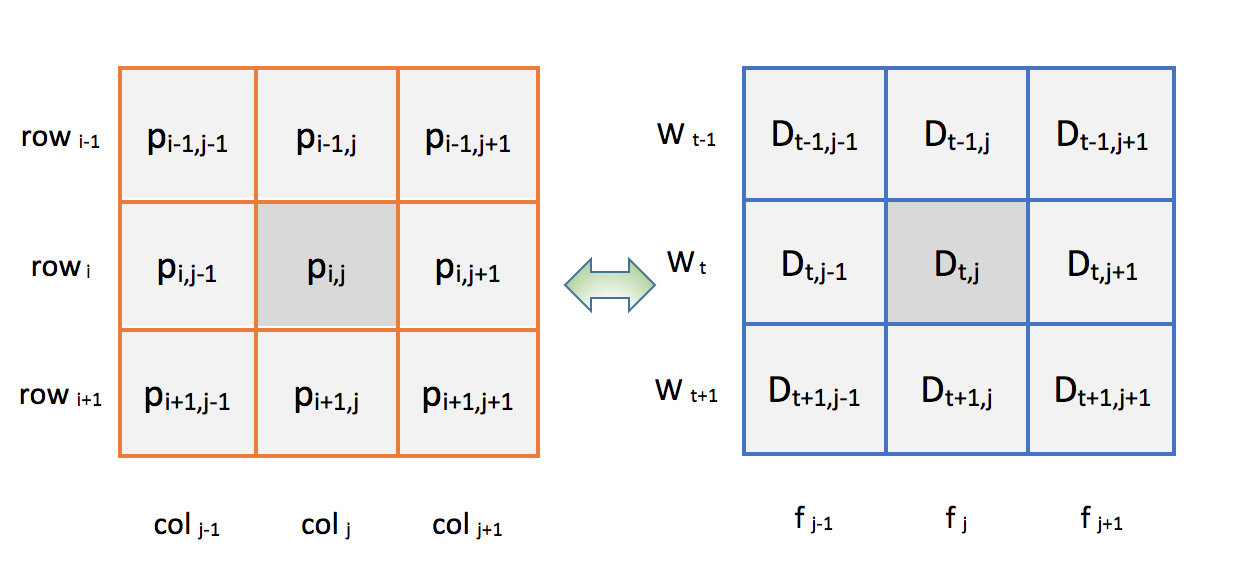
\includegraphics[scale=0.7]{figures/imagebike.png}
\end{adjustbox}
\end{figure}


In an image analysis problem, image samples contains many many pixels and these pixels are surrounded by a lot of pixels that has influence on the target pixel. For a $3\times3$ example as shown in the left sub figure of figure~\ref{imagebike} a target image pixel $p_{i,j}$ is bounded by the related pixels. In this sub figure the rows are mentioned as $i$ and columns as $j$. 

Likewise, for our model to forecast demand in a particular hour $D_{t,j}$ , which is surrounded by some historical hour values as shown in the combined hours field of Table~\ref{datacombo}. So, the demand $D_{t,j}$ is then relies on the combined related feature value $W_t$ (at time t) and $f_j$ is factor $j$. Proposed CNN model is then applied to this time series feature data by reflecting the relations with the image sample and thus dealing this bike rental demand forecasting as an image processing problem. 




\subsection{Model Structure}
\label{structure}

To build the forecasting model to estimate hourly rental bike demand a Convolutional Neural Network model is applied. The structure of a CNN based regression model is shown in figure~\ref{Framework}.


\begin{figure}
\centering
\begin{adjustbox}{addcode={\begin{minipage}{\width}}
{\caption{Structure of a CNN based regression model } 
\label{Framework}
\end{minipage}}}
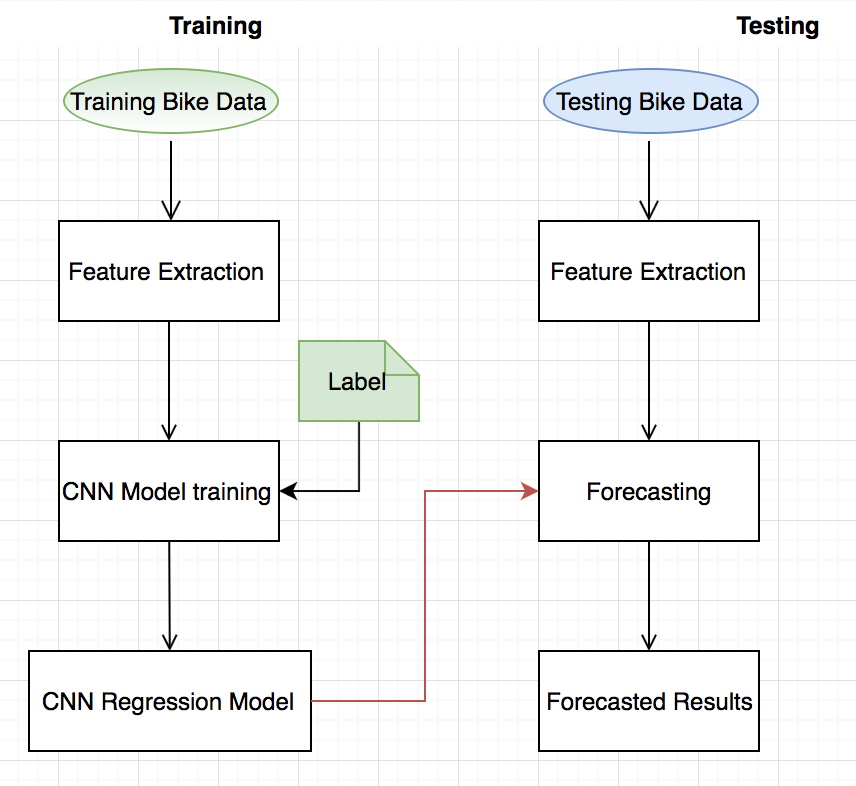
\includegraphics[scale=0.7]{figures/Framework.png}
\end{adjustbox}
\end{figure}


Like any other machine learning method there are two different fragment of it, one is training and the other is testing. For the training part, the datasets gets isolated by keeping the related fields which affects the bike rental demands as features through the feature extraction methods. Afterwards, multiple structures of CNN is analyzed in order to find the best structure of the model. Three different structures of CNN is applied with different convolutional layer count shown in figure~\ref{CNN1}, figure~\ref{CNN2} and figure~\ref{CNN3}. In the next section, this model is implemented on the testing set to forecast the hourly rental demand and then evaluated with four different evaluation matrices to calculate their effectiveness. 



\begin{figure}
\centering
\begin{adjustbox}{addcode={\begin{minipage}{\width}}
{\caption{5 Layer CNN } 
\label{CNN1}
\end{minipage}}}
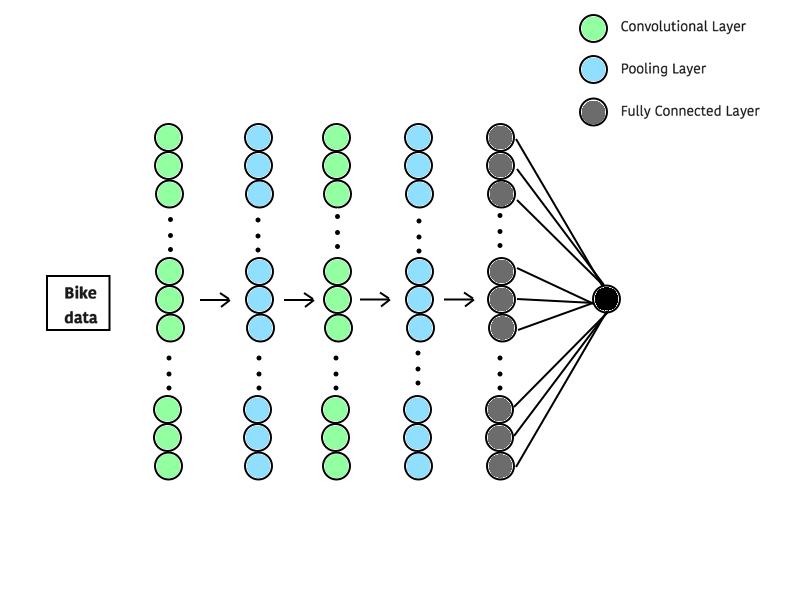
\includegraphics[scale=0.4]{figures/cnn5.png}
\end{adjustbox}
\end{figure}

\begin{figure}
\centering
\begin{adjustbox}{addcode={\begin{minipage}{\width}}
{\caption{6 Layer CNN } 
\label{CNN2}
\end{minipage}}}
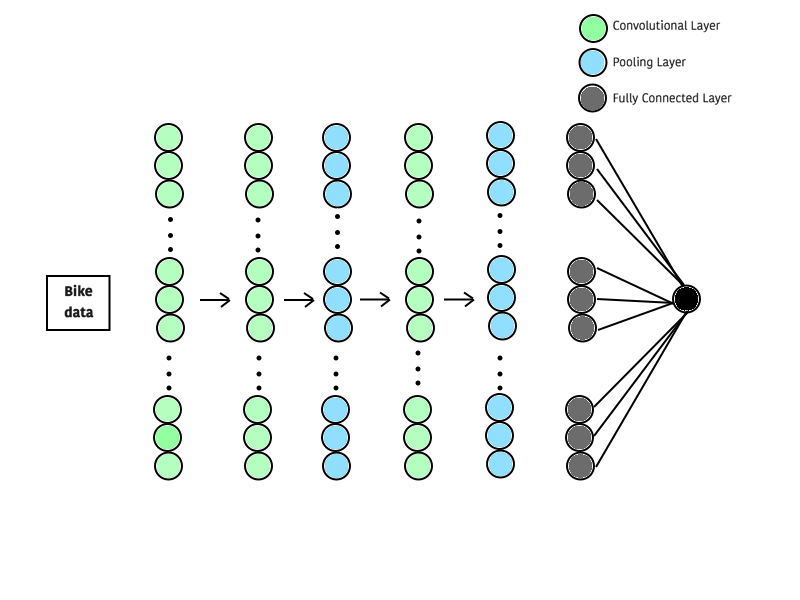
\includegraphics[scale=0.4]{figures/cnn6.png}
\end{adjustbox}
\end{figure}


\begin{figure}
\centering
\begin{adjustbox}{addcode={\begin{minipage}{\width}}
{\caption{7 Layer CNN } 
\label{CNN3}
\end{minipage}}}
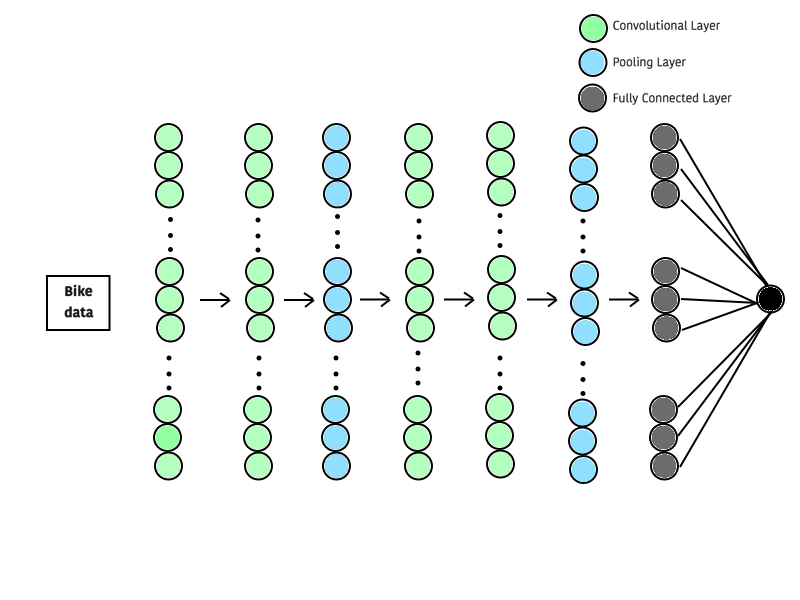
\includegraphics[scale=0.4]{figures/cnn7.png}
\end{adjustbox}
\end{figure}

In figure~\ref{CNN1} there are 5 layers in that CNN structure where, one convolutional layer is connected to one pooling layer which is then connected to another convolutional layer and then again to another pooling layer and finally to a fully connected layer. In figure~\ref{CNN2} there is one extra convolutional layer and in figure~\ref{CNN3} two extra convolutional layer from the 5 layer CNN and thus constructs 6 Layer CNN and 7 Layer CNN respectively. 














%

%%%%%%%%%%%
%
%As highlighted in the previous chapter, analogous to conditioning in probability, DST also has its conditional notions for evidence updating~\cite{CHRISMAN1995}. In this chapter, the basic conditional notions and their implications are presented providing insight into their behavior and the reason behind the choice of the particularly proposed conditional chosen in this thesis.
%
%
%
%
%The most acknowledged DST conditional notions are the DS conditionals~\cite{SHAFER} and FH conditionals~\cite{FaginH}. Although both methods are similar in some respects, FH conditionals possess more intuitive properties (as will be shown in subsequent sections) applicable for hard/soft fusion applications. 
%
%keywords= \lbrace {data handling;diseases;medical computing;regression analysis;social networking (online);Centers for Disease Control and Prevention;H1N1;ILI activity;Twitter data;autoregression models;flu trend prediction;influenza epidemics;influenza-like illness activity data;public health authorities;social network enabled flu trends framework;Correlation;Data models;Delay;Medical services;Predictive models;Real time systems;Twitter}, 
%doi={10.1109/INFCOMW.2011.5928903.
%
%Furthermore, although not expressly treated in this work, Wickramaratne et al. solved the converse problem determining the events which contributed to a particular conditional result. This is obtained by treating the converse CCT problem~\cite{Wickra4}. This is valuable in analyzing how sensitive the knowledge base is to incoming conditioning evidence.
%
%
%
%\section {Conditional Notion Characterization}
%
%An extensive review  was carried out by Kimala and Yamada on DST and the different conditional notions available in literature~\cite{Kimala2008}. However in any application (including soft/hard data fusion), one must consider the suitability of the conditional notion to be applied. 
%
%
%One driver behind our choice of appropriate DST conditional is the natural transition between the DST conditional and Bayesian conditional notions. This is vital because we expect our fusion strategy to be seamlessly integrated with the several approaches applied for dealing with hard data obtained from sensor networks as these methods are well grounded. However, there has been some works on finding the connection between Bayesian and DS theory~\cite{Pearl:1988}. We will now discuss two DST conditional notions arguably the most popular in literature.
%
%
%\subsection{DS or FH Conditionals?}
%The idea behind the DS conditionals is this: assuming we have access to a mass function $m(\textbf{.})$ and some new evidence signifying the occurrence of an event \textit{A}. Since we are confident this event has occurred, we can represent this event using the mass function with one focal element (\textit{A}), the DS conditional with respect to $A$ is given as $m(\extbf{.} \vert A) = (m \oplus m_{A})(\textbf{.})$, where $\oplus$ is the DCR. Technically, DS conditionals may be seen as an extension of Bayesian conditioning only when all focal elements are singletons, but not in general; a property possessed by most if not all other conditional notions. Furthermore, in applications where contradictory evidence are to be combined (as may be encountered in a battlefield scenario), the DCR will produce counterintuitive results. This is therefore a major drawback to the application of DS conditionals.
%
%A rigorous characterization of FH conditionals  has been carried out in which it they are shown to be a true generalization of the Bayesian conditionals~\cite{Fagin89uncertaintybelief, FaginH}. In the Bayesian context, a probability function  is bounded by its inner and outer measures~\cite{FaginH}. In the DS conditional context the probability function induced by inner and outer measures are the belief and plausibility functions respectively. The connection between both Bayesian and DS notions is immediately apparent; DS notions generalize Bayesian notion since inner and outer measures induced by probability functions `map' to DS theoretic belief and plausibility functions.  The fact that currently, no other conditional possesses this feature ~\cite{Fagin89uncertaintybelief} makes the FH our prime choice for the  hard/soft data fusion framework. In conclusion, the DS conditionals can also be constrained by certain paradoxes like \textit{the sure thing principle}, a constraint the FH conditions are able to circumvent~\cite{FaginH}.
%
%In light of the aforementioned reasons, in the following sections, discussions will be restricted to the FH conditionals and their characterizations only.
%
%\section{Characterizing the Conditional Core}
%
%Here we proceed to introduce the \textit{conditional core theorem} (CCT), which provides a theoretical framework with necessary conditions for an element to belong to the conditional core. 
%
%\subsection{Basics}
%
%%\theoremstyle{definition}
%\begin{definition}{(Inner and Outer Sets).}
%Given a BoE $\mathcal{E} \equiv \lbrace \Theta, \mathfrak{F}_{\Theta}, m_{\Theta(\textbf{.})} \rbrace$, and a conditioning event $A \subseteq \Theta$ satisfying $A \in \^{\mathfrak{F}}_\Theta$, the inner and outer sets are defined thus:
%\begin{eqnarray}
%in(A) &\equiv& \{B \subseteq A \vert B  \in  \mathfrak{F} \} \quad and \\
%out(A) &\equiv& \{B \subseteq A \vert B \cup C \in \mathfrak{F}, \quad \emptyset \neq B, \quad \emptyset \neq C \subseteq \overline A\}.
%\end{eqnarray}
%
%\end{definition}
%
%respectively. Also Also for indexes $\mathcal{I}$ and $\mathcal{J}$ spanning in$(A)$ and out$(A)$, we may define collections consisting or arbitrary unions of in(A) and out(A) as:
%\begin {eqnarray}
%IN(A) &=& {\{B \subseteq A \vert B = \bigcup_{\substack{
%   i \subseteq \mathcal{I} }} C_i, C_i \in in(A) \}\\
%OUT(A) &=& {\{B \subseteq A \vert B = \bigcup_{\substack{ j \subseteq \mathcal{J} }}, C_j, C_j \in out(A) \}
%\end{eqnarray}
%
%in$(A)$ connotes the set of focal elements contained in $A$, out$(A)$ contains the focal elements that intersect with but are not contained in $A$, IN$(A)$ and OUT$(A)$ contain arbitrary unions of elements of in$(A)$ and out$(A)$ respectively as shown in Figure ~\ref{inOutA}. $in(A)$, $out(A)$ and their union are significant factors contributing to our main result as shall be shown.
%
%\begin{figure}
%\centering
%\begin{adjustbox}{addcode={\begin{minipage}{\width}}
%{\caption{Pictorial representation of in(A) and out(A)~\cite{Wickra4}.}
%\label{inOutA}
%\end{minipage}}}
%\includegraphics[scale=0.8]{figures/inOutA.png}
%\end{adjustbox}
%\end{figure}
%
%
%%\theoremstyle{definition}
%\begin{definition}{(Straddled Mass).}
%Given a BoE $\mathcal{E} \equiv \lbrace \Theta, \mathfrak{F}_{\Theta}, m_{\Theta(\textbf{.})} \rbrace$, and two arbitrary subsets $A\subseteq \Theta$ and $B \subseteq \Theta$, the term:
%\begin{eqnarray}
%$\mathcal{S} (A;B)$  &= \displaystyle \sum_{\substack{\emptyset \neq X \subseteq A; 
%\emptyset \neq Y \subseteq B}}
%{m_{\Theta}(X \cup Y),
%\end{eqnarray}is the ``straddle'' mass, and is the cumulative mass of propositions straddling $A$ and $B$. 
%\end{definition}
%
%\begin{definition}{(Conditional Belief).}
%The conditional belief of any arbitrary proposition/hypothesis $B \subseteq \Theta$ is given by:
%\begin{eqnarray}
%Bl_{\Theta}(B \vert A) = \frac{Bl_{\Theta}(A \cap B)}{Pl_{\Theta}(A) - \mathcal{S}(\overline{A}; A \cap B)}
%\end{eqnarray}
%
%\end{definition}
%$A$ denotes the conditioning event satisfying $A \in \^{\mathfrak{F}}_{\Theta}$. The proof of this can be inferred from the relationship $Pl_{\Theta}(A) - \mathcal{S}(\overline{A}; A \cap B) = Bl_{\Theta}(A \cap B) + Pl_{\Theta}(A \cap \overline{B})$.
%
%
%\subsection{Conditional Core Theorem (CCT)}
%Having introduced the basics, we now introduce the theorem which specifies the constraints necessary to ascertain whether an element belongs to the conditional core:
%
%\begin{theorem}[Conditional Core Theorem]
%\label{CCT}
%For an arbitrary BoE $\mathcal{E}_{\Theta} = \lbrace \Theta, \mathfrak{F}_{\Theta}, m_{\Theta}(\textbf{.}) \rbrace$, the conditional mass function $m_\Theta(\textbf{.} \vert A)$  must satisfy the following constraints:
%\begin{eqnarray}
%m_{\Theta}(B \vert A) > 0 \leftrightarrow B \in in(A) \quad \textit{or} \\\nonumber
%B \in in(A) \cup OUT(A);
%\end{eqnarray}
%
%where $A$ defines our conditioning event satisfying $A \in \^{\mathfrak{F}}_{\Theta}$.
%\end{Theorem}
%
%This formulation is intuitive because it breaks down the FH notion and   provides insight into the generation of conditional focal elements, and also contains the tools needed to understand how the structure of the core affects the conditional core. The proof of the CCT is however not at all trivial and is hence not included in this thesis. The reader is referred to~\cite{Wickra3} where a through proof is detailed.
%
%Here, a short application example is employed to further expatiate on the CCT. Considering a variation of the illustration in~\cite{Wickra4}, we assume a situation assessment problem where objects that cross the perimeter of a military facility are to be identified. The objects of interest include:
%
%\begin{center}
%
%F \equiv Fighter; M\equiv Bomber;   T \equiv Tank;   S \equiv Soldier;   O \equiv Other
%\end{center}
%
%Furthermore, each class (with exception of $O$) can be subdivided as either $F \equiv Friendly$ or $E \equiv Enemy$ resulting in the following $FOD$
%
%\begin{center}
%$\Theta = \{F_E, F_F, M_E, M_F, T_E, T_F, S_E, S_F, O\}$
%\end{center}
%
%where for instance, $F_e \equiv \textit{enemy fighter jet}, M_f \equiv \textit{friendly bomber} \dots $
%
%BoE  = $\mathcal{E} = \{\Theta, \mathfrak{F} ,m\}$ is the available evidence, where:
%
%\begin{center}
%$\mathfrak{F} = \{M_E, M_F, S_F, (F_E, S_E), (M_E, T_E, O), \Theta \};$
%
%$m(B) = \{0.1, 0.1, 0.1, 0.2, 0.2, 0.3\}.$
%\end{center}
%
%Hence, the core of our BoE on ground, $\mathfrak{F}$, consist singleton propositions like $M_f$ signifying \textit{friendly bomber} and some composite statements like $\lbrace F_e, S_e \rbrace$ signifying \textbf{either}  \textit{enemy fighter jet} \textbf{or} \textit{enemy soldier}.
%
%\begin{table}
%\caption{Table showing conditional elements with non-zero mass. The conditional masses are generated via computation of the mass function given the conditioning event $A=\lbrace F_E , F_F , M_E , M_F , O\rbrace$}.
%\label{example}
%\centering
%\begin{tabular}{||c|c ||c |c||}\hline
%$B$ & $m(B\vert A)$  &  $B & $m(B\vert A)$  \\\hline\hline
%$M_E $&1/9 &$ (M_F, F_E)$& 2/63$ \\
%$M_F$ &1/9 & $(M_E,O)$ & 2/63 \\
%$(M,O)$ &2/63&  $(F_E,M,O)$ & 8/315$\\
%$(M_E,F_E)$ &  2/63 & $(M_E,F_E,O)$& 8/315 \\
% $A $ & 3/5 & &\\\hline
%\end{tabular}
%\end{table}
%
%Assuming we need to update the BoE to reflect incoming intelligence  of $(A = F,M,O)$ supporting  aerial intruder/objects. First we derive:
%$$ in(A) = \lbrace M_E, M_F \rbrace $$
%$$ out(A) = \lbrace F_E. (M_E,O), (F,M,O) \rbrace $$
%$$ IN(A) = \lbrace M_E, M_F, M \rbrace $$
%$$ OUT(A) = \lbrace F_E, (M_E, O), (F_E, M_E,O), (F,M,O) \rbrace $$
%
%Furthermore
%$$ \mathcal{B} = \lbrace (F_E,M_E), (F_E, M_F), (M_E, O), (F_E, M_E, O), (M, O), (F_E, M, O), A \rbrace $$ represents the set of propositions that can be found in $X \cup Y$ where $X \in in(A), Y \in OUT(A)$. Therefore based on the CCT, the concatenation of $\mathcal{B}$ and $in(A)$ constitutes the conditional focal elements, $\mathfrak{F}_{\vert A}$ (i.e. $\lbrace X \subseteq \Theta  \vert X \in in(A)$ or $X \in \mathcal{B} \rbrace $. Table ~\ref{example} shows the computed conditional masses using the CCT. From the above example, some inferences can be made:
%
%\begin{enumerate}
%\item When the evidence on ground $(B)$ is conditioned with $A = (F,M,O)$; hypotheses in favor of only aerial objects stay in the conditional core (e.g. $M_E$), whereas hypothesis supporting non-aerial objects  (e.g. $S_F$) are 'marginalized' out of the conditional core.
%
%\item Regarding the generated conditional focal set:
%	\begin{enumerate}
%	\item The propositions $\{F_E, S_E\}$ and $\{F_E, M_F\}$ receive the unconditioned mass of proposition $\{F_E, S_E\}$
%	\item The reason why generated the mass of $\{F_E, S_E\}$ does not move into just $F_E$ is because our unconditioned core $			\mathfrak{F}$ does not contain any singleton propositions favoring $F_E$, the same can be said for $\{F_E, M_E, O\}$. However 		propositions $F_E$ and $\{M_E, O\}$ do transition into $\{M_E, F_E, O\}$
%	\end{enumerate}
%\end{enumerate}
%
%The intuitiveness of the CCT is immediately apparent, as it shows the  logical coherence behind the allocation of conditional masses. Suppose the conditioning event was more precise (e.g. $A = \lbrace F,M_E, O\rbrace$), we would obtain the following:
%
%$$ in(A) = \lbrace M_E \rbrace $$
%$$ out(A) = \lbrace F_E. (M_E,O), (F,M_E,O) \rbrace $$
%$$ IN(A) = \lbrace M_E \rbrace $$
%$$ OUT(A) = \lbrace F_E, (M_E, O), (F_E, M_E,O), (F,M_E,O) \rbrace $$
%$$ \mathcal{B} = \lbrace (F_E,M_E),  (M_E, O), (F_E, M_E, O), (F, M_E, O) \rbrace $$
%$$\mathfrak{F}_{\vert A} = \lbrace M_E, (F_E,M_E),  (M_E, O), (F_E, M_E, O), (F, M_E, O) \rbrace $$
%
%
%Table~\ref{exampleb} shows the computed conditional masses. It is observed that the focal elements further reduce because the conditioning event has become more precise.
%\begin{table}
%\caption{Table showing conditional elements with non-zero mass and conditional masses are generated given more precise conditioning event $A=\lbrace F_E , F_F , M_E ,O\rbrace$ }
%\label{exampleb}
%\centering
%\begin{tabular}{||c|c ||c |c||}\hline
%$B$ & $m(B\vert A)$  &  $B & $m(B\vert A)$  \\\hline\hline
%$M_E $&0.125 &$ (M_E, F_E)$& 0.04167$ \\
%$(M_E,O)$ &0.04167 & $(F_E,M_E,O)$ & 0.04167 \\
%$A$ &0.75&  $Others$ & 0.000 $\\\hline
%\end{tabular}
%
%\end{table}

%%%%%%%%%%%%%%%%%%%%%%%%%%%%%%%%%%%%%%%%%%%%%%%%%%%
%
%  New template code for TAMU Theses and Dissertations starting Fall 2012.  
%  For more info about this template or the 
%  TAMU LaTeX User's Group, see http://www.howdy.me/.
%
%  Author: Wendy Lynn Turner 
%	 Version 1.0 
%  Last updated 8/5/2012
%
%%%%%%%%%%%%%%%%%%%%%%%%%%%%%%%%%%%%%%%%%%%%%%%%%%%
%%%%%%%%%%%%%%%%%%%%%%%%%%%%%%%%%%%%%%%%%%%%%%%%%%%%%%%%%%%%%%%%%%%%%%
%%                           SECTION V
%%%%%%%%%%%%%%%%%%%%%%%%%%%%%%%%%%%%%%%%%%%%%%%%%%%%%%%%%%%%%%%%%%%%%

\chapter{\uppercase{Experiment \& Results}}

\label{sec:results}



\section{Dataset Combination \& Feature Selection}
\label{Datacombination}

In order to apply machine learning algorithm to forecast bike rental demand effectively, important features from the datasets (City bike trip data, Weather data, Holiday data) needs to be collected. From the target dataset mentioned earlier in this thesis, the common fields like `year', `month', `day', `hour' counted once. Alsothose bike data contains more than $3$million rental data, male data is about 2,342,359 and female data is about 651,398 and rest is unknown gender data. These bike rental data is then combined with the weather and holiday data as shown in Table~\ref{datacombo}. `Feature no.' field shows the number of features related to the second column which is the name of the feature. Then Table~\ref{datacombo} also shows the type of the features (numeric or binary), source of the features (1= city bike trip data, 2= weather data, 3= holiday data) and the combined hours means the hour numbers combined together to build the dataset. For example, 1-8 feature is about the hourly rental count, which is a numeric data, for combined hours field hour -1 is the previous hour data, -24 is the data from 24 hours earlier and so on. 



\begin{table}[]
\centering
\caption{Feature selection}
\label{datacombo}
\begin{tabular}{||l|l|l|l|l||}
\hline
Feature no. & Name                  & Type    & Combined hours                      & Source \\ \hline \hline
1-8         & Hourly rental count   & numeric & -1,-24,-48,-72,-96,-120,-144,-168 & 1      \\ \hline
9-16       & Age                   & numeric & -1,-24,-48,-72,-96,-120,-144,-168 & 1      \\ \hline
17-24       & Trip duration         & numeric & -1,-24,-48,-72,-96,-120,-144,-168 & 1      \\ \hline
25-32       & Bike count            & numeric & -1,-24,-48,-72,-96,-120,-144,-168 & 1      \\ \hline
33-40       & Month                 & numeric & -1,-24,-48,-72,-96,-120,-144,-168 & 1      \\ \hline
41-48       & Day                   & numeric & -1,-24,-48,-72,-96,-120,-144,-168 & 1      \\ \hline
49-56       & Snow depth            & numeric & -1,-24,-48,-72,-96,-120,-144,-168 & 2      \\ \hline
57-64       & Snow fall             & numeric & -1,-24,-48,-72,-96,-120,-144,-168 & 2      \\ \hline
65-72      & Wind speed            & numeric & -1,-24,-48,-72,-96,-120,-144,-168 & 2      \\ \hline
73-80       & Temperature          & numeric & -1,-24,-48,-72,-96,-120,-144,-168 & 2      \\ \hline
81-88       & Precipitation         & numeric & -1,-24,-48,-72,-96,-120,-144,-168 & 2      \\ \hline
89-96     & Holiday               & binary  & -1,-24,-48,-72,-96,-120,-144,-168 & 3      \\ \hline
97-104     & Weekday               & binary  & -1,-24,-48,-72,-96,-120,-144,-168 & 3      \\ \hline
105-112    & Weekend (not holiday) & binary  & -1,-24,-48,-72,-96,-120,-144,-168 & 3      \\ \hline
\end{tabular}
\end{table}


\section {Baseline Algorithms}
\label{BaseAlgos}

In order to compare the results of proposed method some baseline models are chosen. These are- Linear regression, Neural network, Support vector regression (SVR) which are very popular and very effective machine learning algorithms in recent time. A brief description about this algorithms are given below in order to understand the methods better and how it compares to our model. 

\subsection{Linear Regression}
\label{LR}

Regression is  one of the most widely used models in recent years according to ~\cite{seber2012linear}. This algorithm assumes that the target variable $y$ on features $x_1,x_2,x_3 ... x_n$ is linear, thus it tries to find the best suitable model to fit the target. This model is then used to do prediction ~\cite {han2011data}. 

\begin{figure}
\centering
\begin{adjustbox}{addcode={\begin{minipage}{\width}}
{\caption{Simple Linear Regression~\cite{wang2016forecasting}}  
\label{linear}
\end{minipage}}}
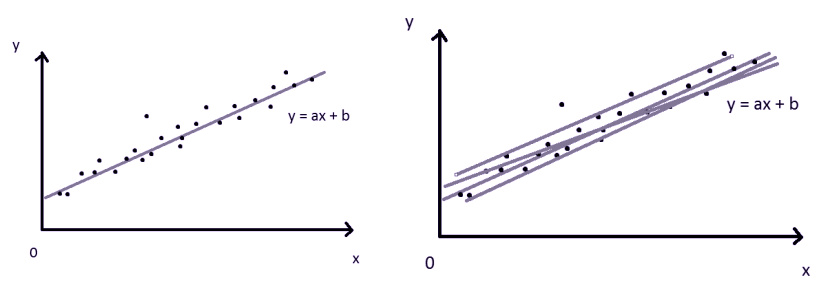
\includegraphics[scale=0.4]{figures/linear.png}
\end{adjustbox}
\end{figure}

From the figure~\ref{linear} we can see a simple example of linear regression. For two variable $x  \&  y$ and the relationship between them is $y=ax+b$. From this example at any given value of $x$, dependent variable $y$  can be predicted . But many lines can fit the model perfectly, for which residuals should be taken into count. Suppose if,  $A(x_1,y_1)$ using $y=ax+b$ can predict $A^\prime(x_1,ax_1+b) $ then the disparity between $A$ and $A^\prime$ is called residual ~\cite{montgomery2012wiley}. The residual sum of squares, $ RSS = (y_1-ax_1-b)^2 +(y_2 - ax_2 - b )^2 + ... + (y_n-ax_n-b)^2)$ [figure~\ref{linear2}].


\begin{figure}
\centering
\begin{adjustbox}{addcode={\begin{minipage}{\width}}
{\caption{Residual example~\cite{wang2016forecasting}}  
\label{linear2}
\end{minipage}}}
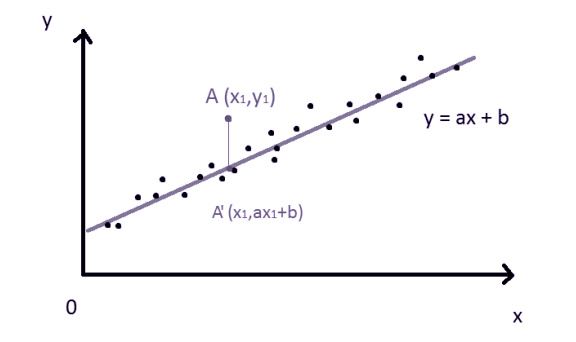
\includegraphics[scale=0.4]{figures/linear2.png}
\end{adjustbox}
\end{figure}



\subsection{Neural Network}
\label{NN}

Neural network is currently one of the most discussed and most commonly used machine learning algorithm. It is getting more and more attention from the researchers all over the world~\cite{rojas2013neural}. Its methodology is based on animal neurons, with a joined assembly of simple elements. The internal connection strengths ensures the processing ability of the network or weights which is obtained through learning~\cite{gurney1997introduction}. 

According to~\cite{rojas2013neural} an abstract neuron [figure~\ref{NN1}] can have $n$ inputs. Each input frequency t can convey $x_t$ information, weight $w_t$ and $f$ being the primitive function. The transmitted information is integrated at the neuron and the primitive function is then evaluated~\cite{rojas2013neural}.

\begin{figure}
\centering
\begin{adjustbox}{addcode={\begin{minipage}{\width}}
{\caption{Abstract neuron~\cite{rojas2013neural}}  
\label{NN1}
\end{minipage}}}
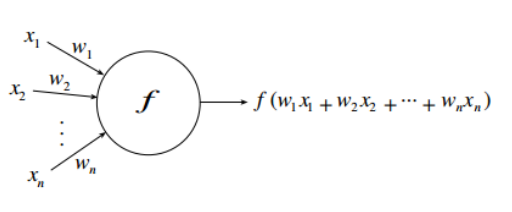
\includegraphics[scale=1.2]{figures/NN1.png}
\end{adjustbox}
\end{figure}


Neural network has the ability to combine $n$ basic functions. In figure~\ref{NN2} four functions $f_1,  f_2, f_3, f_4$, network function  $ \Phi $  is estimated at the point $x, y, z$. Weights $ \alpha_1, \alpha_2,… \alpha_5 $ can also create different network functions.





\begin{figure}
\centering
\begin{adjustbox}{addcode={\begin{minipage}{\width}}
{\caption{Functional model of a Neural Network~\cite{rojas2013neural}}  
\label{NN2}
\end{minipage}}}
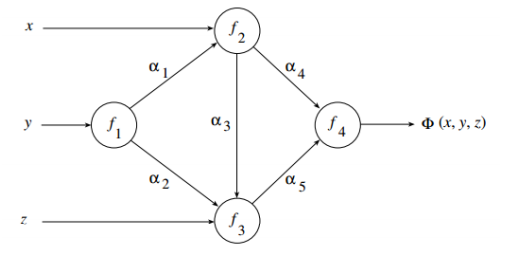
\includegraphics[scale=1.2]{figures/NN2.png}
\end{adjustbox}
\end{figure}

\subsection{Support Vector Regression}
\label{SVR}

Support vector machine (SVM) is a very powerful and widespread supervised machine learning model~\cite{friedman2001elements} which are used to solve regression or classification problems. The version of it that deals with regression is known as Support Vector Regression (SVR). SVR is commonly known for its high level of generalization, therefore, this model can be used in new, previously unobserved data with high accuracy. In SVR figure~\ref{NN2}, support vectors fabricated on the $\epsilon$ tube bounding decision shell, called training samples. Residuals which are fewer than $\epsilon$ has no influence on predictions.

\begin{figure}
\centering
\begin{adjustbox}{addcode={\begin{minipage}{\width}}
{\caption{Non-linear SVR ~\cite {jain2014forecasting}  }  
\label{SVR}
\end{minipage}}}
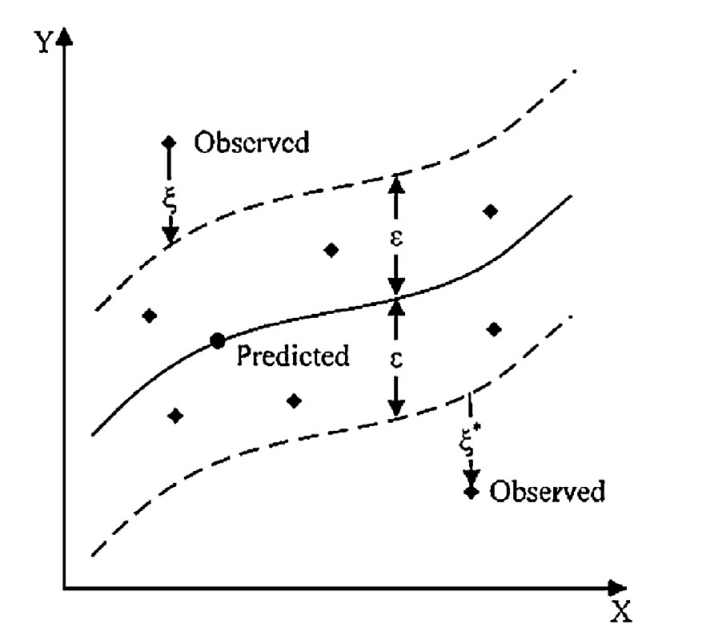
\includegraphics[scale=0.7]{figures/SVR.png}
\end{adjustbox}
\end{figure}


Suppose, for a given dataset ${(X_i, Y_i)}^{i=N} _{i=1}$, where input variables X and output Y, SVR estimates the relationship as : 

$Y - W.\Phi (X)+b$ , here $\Phi (X)$ is a non-linear kernel function which non-linearly maps from the input space X to the feature space. By minimizing the following function coefficients W and b are determined :


$min  {\frac{1}{2}}\parallel w\parallel ^{2} + C\frac{1}{N}\sum_{i=1}^{N}\xi _i+\xi _i^*$

with constraints –


$Y_i - W.\Phi (X_{i})-b\leq \epsilon +\xi _{i}$

$W.\Phi (X_{i})+b-Y_{i}\leq \epsilon +\xi _{i}^*$

$\xi ,\xi _{i}^*\leq0$

Here, to attain acceptable results $W$ the weight should be as flat as achievable. $\xi _{i}$ $ \xi _{i}^*$ are the residuals beyond $\epsilon $ and the regularization parameter is the cost $C$. 




\section{Evaluation Metrices}
\label{Evaluation}

In order to assess the model accuracy, this work uses four evaluation metrices. Mean absolute percentage of error (MAPE), Root-mean-square error (RMSE), normalized Mean absolute error (NMAE), and Normalized root-mean-square error (NRMSE). 

MAPE metric has been used in a amount of prediction studies~\cite{ hu2015mid}~\cite{edwards2012predicting}. It describes the average absolute error as percentage by the following equation-

$MAPE = \frac{1}{N}\sum^{N}_{i=1}(\left | \frac{y_i - \hat y_i}{y_i} \right |\times 100)$

Here, $y_i$ is the actual value,  $ \hat y_i $ is the predicted value and $N$ being the number of observations. The value of MAPE relies on the score and the lower the score is higher the performance is. MAPE value for lower forecast can not exceed $100 \%$, but there is no limit for higher forecasts.  MAPE can also not be used if there are zero values as it will be divided by zero. 

RMSE depends on the measure of the variables and should be used to compare forecasting for the similar series across the models as relative measure. Similar to MAPE, the smaller the error better the forecasting. 

$RMSE = \sqrt[]{\frac{1}{N}\sum_{i=1}^{N}(\hat y_i - y_i)^2}$

One issue with evaluating with RMSE is the forecast error varies across time. Non- linearity in the model or deviations in exogenous variables can cause this issue. According to~\cite{fair1990comparing} no severe statistical analysis can be put on the RMSE because they are not approximations of any factor in the model. 


NMAE measure normalizes the mean absolute error by the range of possible data values. NMAE is defined as follows- 


$ NMAE=\frac{\sum_{i=1}^{N}(\left |  \hat y_i-y_i\right |)}{\sum_{i=1}^{N}(\left |  y_i\right |)}$

NRMSE is the normalized root mean square error which compares between models with different scales. Similar to RMSE the value is expressed as percentage and lower value means less residual differences. 

$  NRMSE=\sqrt[]{\frac{\sum_{i=1}^{N}(  \hat y_i-y_i)^2}{\sum_{i=1}^{N}(  y_i)^2} }$ \\

%\subsection{Tensorflow}
%\label{Tensorflow}
%
%For implementing the Convolutional Neural Network, Tensorflow- an open source software for the numerical computation using data flow graphs is used ~\cite{tensorflow}. In Tensorflow the nodes represents the mathematical operations and graph edges represents the tensors (multi dimensional data arrays) between them. The advantages of using Tensorflow is to apply computation to one or more CPU’s or GPU’s with a single API. 




\section {Results}
\label {results}


This section focuses on how the proposed CNN model is actually performing against the three baseline models (Linear regression, Neural Network, SVR). As mentioned earlier Table~\ref{datacombo} we selected the features from those three datasets and created the time series featureset. The featureset contains $9\times14$, total $126$ features which has current hour data as well as 8 previous hours data based on the Table~\ref{datacombo}. Two different training and testing dataset were created based on monthly bike rental demand records. These dataset counts are also shown in Table~\ref{dataset}.  Proposed model CNN is used from Tensorflow with the parameter estimation of AdomOptimizer, filter $3\times 3 $, max pooling size $2 \times 2$.  

%%%%

\begin{table}[]
\centering
\caption{Dataset counts}
\label{dataset}
\begin{tabular}{||c|l||c|l||}
\hline
\multicolumn{2}{||c||}{Training set}                     & \multicolumn{2}{c||}{Testing set} \\ \hline \hline
\multicolumn{1}{||l|}{Male} & Female                    & Male  & Female                   \\ \hline
3612                       & \multicolumn{1}{c||}{3529} & 720   & \multicolumn{1}{c||}{714} \\ \hline
\end{tabular}
\end{table}

%%%%



\section {Discussion}
\label {Discussion}

From the results in Table~\ref{femalecomp} and Table~\ref{malecomp} we can see the comparison between methods for forecasting bike rental demand for both female and male. Comparing CNN with other methods for both genders shows that CNN outperforms other baseline models with significant advantages constantly in all four different metrices. It also shows that results gained from the male datasets are far superior than the result gained from female datasets. MAPE results gained for female varies from 8-12 \% for baseline models where CNN shows 7 \%. It also shows better percentage level for male dataset where CNN is only 3-4 \%. The reason for male data to show better forecasting results is because there are a lot of data available for male users as shown in the figure~\ref{genderpie}. As the results from those two table showing CNN is performing better than the baseline models it is understandable that the goal of the thesis and the methodology used to achieve this, is proving to be effective. 

Even though CNN results are better than baseline models it is still confusing to decide which structure of CNN should be used. For female dataset 5 layer CNN is working better than others where in male dataset 7 layer CNN is working better. In overall, treating this bike rental data as an image processing sample and doing demand forecasting of hourly rental bike demand using CNN is a successful demand forecasting technique. 

% Please add the following required packages to your document preamble:
% \usepackage{multirow}
\begin{table}[]
\centering
\caption{Comparison of results between proposed and baseline models (Female dataset)}
\label{femalecomp}
\begin{tabular}{|c|c|c|c|c|}
\hline
\multirow{2}{*}{Model Name} & \multicolumn{4}{c|}{Dataset Used - Female}                                                                              \\ \cline{2-5} 
                            & \multicolumn{1}{l|}{MAPE} & \multicolumn{1}{l|}{NMAE} & \multicolumn{1}{l|}{RMSE} & \multicolumn{1}{l|}{NRMSE} \\ \hline
Linear Regression            & 8.987                     & 0.062                     & 0.509                     & 0.084                      \\ \hline
Neural Network              & 11.263                    & 0.084                     & 0.677                     & 0.112                      \\ \hline
SVR                         & 8.869                     & 0.084                     & 0.052                     & 0.085                      \\ \hline
5 Layer CNN                 & \textbf{7.373}            & 0.051                     & \textbf{0.327}            & \textbf{0.045}             \\ \hline
6 Layer CNN                 & 7.654                     & \textbf{0.050}            & 0.043                     & 0.073                      \\ \hline
7 Layer CNN                 & 7.489                     & \textbf{0.050}            & 0.425                     & 0.070                      \\ \hline
\end{tabular}
\end{table}

%%%%
\begin{table}[]
\centering
\vspace{1ex}
\caption{Comparison of results between proposed and baseline models (Male dataset)}
\label{malecomp}
\begin{tabular}{|c|c|c|c|c|}
\hline
\multirow{2}{*}{Model Name} & \multicolumn{4}{c|}{Dataset Used - Male}                                                                       \\ \cline{2-5} 
                            & \multicolumn{1}{l|}{MAPE} & \multicolumn{1}{l|}{NMAE} & \multicolumn{1}{l|}{RMSE} & \multicolumn{1}{l|}{NRMSE} \\ \hline
Linear Regression            & 4.330                     & 0.038                     & 0.378                     & 0.052                      \\ \hline
Neural Network              & 6.068                     & 0.053                     & 0.548                     & 0.075                      \\ \hline
SVR                         & 4.529                     & 0.039                     & 0.408                     & 0.056                      \\ \hline
5 Layer CNN                 & 4.059                     & 0.036                     & 0.361                     & 0.049                      \\ \hline
6 Layer CNN                 & 4.031                     & 0.036                     & 0.347                     & 0.048                      \\ \hline
7 Layer CNN                 & \textbf{3.531}            & \textbf{0.030}            & \textbf{0.327}            & \textbf{0.045}             \\ \hline
\end{tabular}
\end{table}

%%%%%%%%%%%%%%%%%%%




%%%%%%%%%%%%%%%%%%%%%%%%%%%%%%%%%%%%%%%%%%%%%%%%%%%
%
%  New template code for TAMU Theses and Dissertations starting Fall 2012.  
%  For more info about this template or the 
%  TAMU LaTeX User's Group, see http://www.howdy.me/.
%
%  Author: Wendy Lynn Turner 
%	 Version 1.0 
%  Last updated 8/5/2012
%
%%%%%%%%%%%%%%%%%%%%%%%%%%%%%%%%%%%%%%%%%%%%%%%%%%%

%%%%%%%%%%%%%%%%%%%%%%%%%%%%%%%%%%%%%%%%%%%%%%%%%%%%%%%%%%%%%%%%%%%%%%%
%%%                           SECTION II
%%%%%%%%%%%%%%%%%%%%%%%%%%%%%%%%%%%%%%%%%%%%%%%%%%%%%%%%%%%%%%%%%%%%%%

\chapter{\uppercase { Conclusion \& Future work}}

\label{Conclusion}

This chapter will review the whole thesis and summarize the current need of demand forecasting and the approach of bike sharing service demand forecasting. Few future work and research will also be mentioned. 


\section {Conclusion}
\label{conclusion}

In the years to come ``Big Data" term will continue to grow bigger and bigger, which makes it essential for companies to embrace this challenge with open arms and learning, implementing the required skills to tackle this. This thesis, which is mainly focuses on the demand forecasting in different fields, first recognized few challenges it poses and showing potential of using it for the benefit of organizations. It also a must to dedicate enough time and resources to be able to overcome the issues. 




This thesis is specially looking at a particular transportation demand forecasting by doing hourly bike rental demand forecasting where the idea of the topic came from winning the Big data competition where the main goal was to improve the bike share program (as mentioned earlier). In order to do the bike rental demand forecasting first we did some statistical analysis on the bike rental data. From those analyses it is found that there is a big prospective of trying to attract more female users in to this bike share program. Also the visualization of the different factors of the data also showed customers mainly uses bike share program for doing short trips which makes it very important to have rentable bikes available or free parking spaces in the stations whenever customer wants. For the first problem, different types of bikes according to gender preference and forecasting hourly rental bike demand using CNN is for the latter problem is proposed. The main contribution of this thesis is from the results gained from the experiment, which proves that doing forecasting using CNN and treating bike samples as image samples to solve regression problem is a very reasonable and achievable way to deal with the problems stated above. Nevertheless, CNN performs better than the baseline models but it is not significant. Reason being the lack of datasets may reduce the performance of the overall model. 

\section{Future Work}
\label{future}

There are many additional work can be done in this topic as demand forecasting is proving to be one of the most important area for many organizations. 

In future a demand forecasting experiment on the health care program can be carried out as it is also a very important section of demand forecasting. 

For the transportation demand forecasting in bike share program, there are too many factors which may cause variance in user's behavior such as - biking events or marathon, extremely snowy day or tornado, government restriction regarding traffic. Therefore, it is almost impossible to consider all the factors in one research, thus, this thesis focuses on building a model to forecast the hourly rental bike demand to predict the number of rental demand in future based on the historical data of bike rentals, weather and holiday data. So separating every docking stations and treating them individually and forecasting their rental demands can be another very useful way to solve this problem. 

The results also showed inconsistency between the different layers of CNN so finding the best structure needed for the different datasets is also a very important task to work on. It is also possible to implement transfer learning on the bike rental data forecasting model from another transportation forecasting model such as taxi or uber data. Maybe doing this we can get more insights on the users behavior which will make our model more useful. 

Finally, ``Big Data", as we all know the bigger the dataset is better the performance will be. So collecting more data can only improve the forecasting results and predicting accuracy. But it is also important to clear out any noises it may have in a very tactful way to get the best possible results of demand forecasting. 












%%%%%%%%%%%%%%%%%%%%%%%%%%%%%%%%%%%%%%%%%%%%%%%%%%%%
%%
%%  New template code for TAMU Theses and Dissertations starting Fall 2012.  
%%  For more info about this template or the 
%%  TAMU LaTeX User's Group, see http://www.howdy.me/.
%%
%%  Author: Wendy Lynn Turner 
%%	 Version 1.0 
%%  Last updated 8/5/2012
%%
%%%%%%%%%%%%%%%%%%%%%%%%%%%%%%%%%%%%%%%%%%%%%%%%%%%%
%%%%%%%%%%%%%%%%%%%%%%%%%%%%%%%%%%%%%%%%%%%%%%%%%%%%%%%%%%%%%%%%%%%%%%%
%%%                           SECTION VI
%%%%%%%%%%%%%%%%%%%%%%%%%%%%%%%%%%%%%%%%%%%%%%%%%%%%%%%%%%%%%%%%%%%%%%
%
%
%
%\chapter{\uppercase{Conclusions and Future Work}}
%
%\section{Conclusions}
%
%The focus of this thesis has been the development of an efficient algorithm to apply the CCT to identify the conditional focal elements of  FH conditionals and compute their masses, beliefs and store the data required for their graphical representation all in one framework. The binary representation was used. It has been shown that the CCT in most real application will provide computational savings. The criterion for computational savings have also been derived. The structure of the proposed algorithm is such that a lot of optimizations to further reduce computational overhead can be made. This framework will be able to handle conflicting evidence, a problem the traditional combination operator (DRC) cannot circumvent.
%The proposed approach carries a lot of potential to an analyst who may want to determine sensitivity of a knowledge base to incoming evidence, and understand the intuition behind the generation of conditional focal elements.
%
%
%\section{Future Work}
%
%Further work  will be the validation of this algorithm using real data. Although after the data has been preprocessed, both synthetic and real data will typically have the same format, this is still necessary for validation.
%
%
%%Due to the time constraint, some further work was envisaged but could not be carried out. Firstly the simulations were done using synthetic data, one aspect of the further work is to apply real data for validation. Also, considering that soft evidence will have various degrees of reliability, in further work uncertainty modeling framework should be able to account for this.
%
%Another is to optimize the efficiency of this algorithm, by applying more appropriate data structures which will help perform computations with the least amount of  computational resources. In this thesis, only the binary representation was used throughout. This representation is only optimal for looking up a mass function $m(A)$ for a given $A$. Operations  like marginalization, listing of focal sets and conditioning however will take exponential time in $\vert \Theta \vert$. This is unavoidable when $\vert \mathfrak{F} \vert$ is close to $2^{\vert \Theta \vert}$ even though in real problems this is seldom the case. The n-dimensional array therefore does not take advantage of the sparseness of data in these situations.
%
%The ordered list representation on the other hand although is more complicated in value look-up than the n-array representation, permits ``random access'' such that one can access any pair of hypothesis (and mass) without having to visit earlier pairs. This operation (random access) will take log$\vert \mathfrak{F} \vert$ for a single value, log$\vert \mathfrak{F} \vert$ + log$\vert \Theta \vert$ to retrieve a single subset of $A$ and time proportional to $\vert \Theta \vert$ to retrieve all subsets of $A$ (as $log_2 \vert \mathfrak{F} \vert \leq \vert \Theta \vert$).
%
%The binary tree representation, due to its inherent structure will require storage proportional to $\vert \Theta \vert \vert \mathfrak{F} \vert$ and time proportional to $\vert \Theta \vert \vert \mathfrak{F} \vert (log\vert \Theta \vert + log \vert \mathfrak \vert )$ to construct. Although operations like normalizing and  listing and will take slightly longer (by a constant factor) than the ordered list representation, the computation of $m(A)$, and $bel(A)$ (for $A \subseteq \Theta$) will take time proportional to $\vert \Theta \vert$~\cite{implementingbelief}.
%There are also logical representations like the ordinary binary decision diagrams (OBDD). Although one can derive algorithms for all primitive operations (intersection, equality testing, projection, extension) in polynomial time using OBDDs, they have not been applied within DST framework yet. Further work will therefore be to employ the use of such appropriate data structures for further optimization of the proposed algorithm.
%
%
%Thirdly, probabilistic graphical models (PLM) e.g. Bayesian networks, Conditional Random Fields etc., offer significant computational advantages using efficient message-passing approaches as they have within the Bayesian framework. Since the algorithm already stores the data required for graphical representation of conditional focal elements, the application of probabilistic graphical models for efficient computation of masses and belief simultaneously by exploiting the relationship between the conditional focal elements, and ordering the calculations appropriately is an intuitive approach because conditional masses and inferences can be computed simultaneously. The introduction of PLMs will be very beneficial especially when considering appropriate visualization and dealing with problem involving large sets of input data.
%
%Finally, as earlier mentioned, the proposed work was done assuming the soft data has been transformed into a usable format by a natural language processing (NLP) interface. In future work the entire pipeline; from raw data to NLP, to decision level fusion under the DST framework will be considered.
%
%
%
%%%%%%%%%%%%%%%%%%%%%%%%%%%%%%%%%%%%%%%%%%%%%%%%%%%%%%%%
%%\begin{figure}[H]
%%\centering
%%\includegraphics[scale=.50]{figures/Penguins.jpg}
%%\caption{Another TAMU figure}
%%\label{fig:tamu-fig4}
%%\end{figure}
%%%%%%%%%%%%%%%%%%%%%%%%%%%%%%%%%%%%%%%%%%%%%%%%%%%%%%%%
%
%


%fix spacing in bibliography, if any...
%%%%%%%%%%%%%%%%%%%%%%%%%%%%%%%%%%%%%%%%%%%%%%%%%%%%%%%%%%%%%
\let\oldbibitem\bibitem
\renewcommand{\bibitem}{\setlength{\itemsep}{0pt}\oldbibitem}
%%%%%%%%%%%%%%%%%%%%%%%%%%%%%%%%%%%%%%%%%%%%%%%%%%%%%%%%%%%%%%%
%%%%%%%%%%%%%%%%%%%%%%%%%%%%%%%%%%%%%%%%%%%%%%%%%%%
%
%  New template code for TAMU Theses and Dissertations starting Fall 2012.  
%  For more info about this template or the 
%  TAMU LaTeX User's Group, see http://www.howdy.me/.
%
%  Author: Wendy Lynn Turner 
%	 Version 1.0 
%  Last updated 8/5/2012
%
%%%%%%%%%%%%%%%%%%%%%%%%%%%%%%%%%%%%%%%%%%%%%%%%%%%


%%%%%%%%%%%%%%%%%%%%%%%%%%%%%%%%%%%%%%%%%%%%%%%%%%%%%%%%%%%%%%%%%%%%%%
%%                           REFERENCES 
%%%%%%%%%%%%%%%%%%%%%%%%%%%%%%%%%%%%%%%%%%%%%%%%%%%%%%%%%%%%%%%%%%%%%

\phantomsection
\addcontentsline{toc}{chapter}{REFERENCES}
\renewcommand{\bibname}{{REFERENCES}}
%\renewcommand{\bibname}{{\large\textbf\center REFERENCES}}

\bibliographystyle{ieeetr}
\bibliography{references}

%%%%%%%%%%%%%%%%%%%%%%%%%%%%%%%%%%%%%%%%%%%%%%%%%%%%
%
%  New template code for TAMU Theses and Dissertations starting Fall 2012.  
%  For more info about this template or the 
%  TAMU LaTeX User's Group, see http://www.howdy.me/.
%
%  Author: Wendy Lynn Turner 
%	 Version 1.0 
%  Last updated 8/5/2012
%
%%%%%%%%%%%%%%%%%%%%%%%%%%%%%%%%%%%%%%%%%%%%%%%%%%%

\begin{appendices}
\titleformat{\chapter}{\centering\normalsize}{APPENDIX \thechapter}{0em}{\vskip .5\baselineskip\centering}
\renewcommand{\appendixname}{APPENDIX}

%%%%%%%%%%%%%%%%%%%%%%%%%%%%%%%%%%%%%%%%%%%%%%%%%%%
%
%  New template code for TAMU Theses and Dissertations starting Fall 2012.  
%  For more info about this template or the 
%  TAMU LaTeX User's Group, see http://www.howdy.me/.
%
%  Author: Wendy Lynn Turner 
%	 Version 1.0 
%  Last updated 8/5/2012
%
%%%%%%%%%%%%%%%%%%%%%%%%%%%%%%%%%%%%%%%%%%%%%%%%%%%

%%%%%%%%%%%%%%%%%%%%%%%%%%%%%%%%%%%%%%%%%%%%%%%%%%%%%%%%%%%%%%%%%%%%%%
%%                           APPENDIX A 
%%%%%%%%%%%%%%%%%%%%%%%%%%%%%%%%%%%%%%%%%%%%%%%%%%%%%%%%%%%%%%%%%%%%%

\phantomsection

\chapter{\uppercase{First Appendix}}

Text for the Appendix follows.

\begin{figure}[H]
\centering
\includegraphics[scale=.50]{figures/Penguins.jpg}
\caption{TAMU figure}
\label{fig:tamu-fig5}
\end{figure}

%%%%%%%%%%%%%%%%%%%%%%%%%%%%%%%%%%%%%%%%%%%%%%%%%%%
%
%  New template code for TAMU Theses and Dissertations starting Fall 2012.  
%  For more info about this template or the 
%  TAMU LaTeX User's Group, see http://www.howdy.me/.
%
%  Author: Wendy Lynn Turner 
%	 Version 1.0 
%  Last updated 8/5/2012
%
%%%%%%%%%%%%%%%%%%%%%%%%%%%%%%%%%%%%%%%%%%%%%%%%%%%

%%%%%%%%%%%%%%%%%%%%%%%%%%%%%%%%%%%%%%%%%%%%%%%%%%%%%%%%%%%%%%%%%%%%%%
%%                           APPENDIX B
%%%%%%%%%%%%%%%%%%%%%%%%%%%%%%%%%%%%%%%%%%%%%%%%%%%%%%%%%%%%%%%%%%%%%

\chapter{\uppercase {Second Appendix with a longer title - much longer in fact}}

Text for the Appendix follows.

\begin{figure}[H]
\centering
\includegraphics[scale=.50]{figures/Penguins.jpg}
\caption{TAMU figure}
\label{fig:tamu-fig6}
\end{figure}

\section{Appendix Section}


\pagebreak{}

\end{appendices}


\chapter*{CURRICULUM VITA}
\addcontentsline{toc}{chapter}{VITA}  % Needs to be set to part, so the TOC doesnt add 'CHAPTER ' prefix in the TOC.

% Comment the following lines to use the default Computer Modern font
% instead of the Palatino font provided by the mathpazo package.
% Remove the 'osf' bit if you don't like the old style figures.

% Set your name here
\def\name{Safat Mahmood}

% Don't indent paragraphs.
\setlength\parindent{0em}

% Make lists without bullets
\renewenvironment{itemize}{
  \begin{list}{}{
    \setlength{\leftmargin}{1.5em}
  }
}{
  \end{list}
}
% Place name at left
\section*{\large \bf \name}
\begin{singlespace}

\begin{minipage}{0.45\linewidth}
  Prairie View A\&M University \\
  Department of Electrical and Computer Engineering \\
  P.O. Box 519, Prairie View, 77446
\end{minipage}
\begin{minipage}{0.45\linewidth}
  \begin{tabular}{ll}
    Phone: & (713) 377-8388 \\
    Email: & \url{safatmahmood@gmail.com} \\
  \end{tabular}
\end{minipage}


\section*{\large \bf Education}

\begin{itemize}
  \item M.S. Electrical and Computer Engineering, Prairie View A\&M University, 2015.

  \item B.Eng. Electrical/Electronics Engineering, Queen Mary University of London, 2012.

\end{itemize}

\section*{\large \bf Employment}

\begin{itemize}
\item Prairie View A\&M University, Research Assitant, 2015--2016.
\item Pacific Jeans Ltd., Assistant Engineer, 2013-14.
\end{itemize}

\section*{\large \bf Professional Skills}
\begin{itemize}
\item Solid foundation of theoretical knowledge, with sound practical electrical engineering/ programming skills, and strong/quick learning ability.
\item Natural Language Processing (NLP), Information Extraction \& sentiment analysis,Machine learning, Deep learning,Network and Cyber Security,Robotic Sensing, Semiconductors, Microcontrollers
\item Embedded system, assembly language , FPGA, C++, python, Matlab, HTML,CSS and many more.
\end{itemize}

\section*{\large \bf Achievements \& Social works}

%\subsection*{Journal Articles}

\begin{itemize}
%\item Joshua Bassey, Lijun Qian, Alexander Aved, Timothy Kroecker, 
%{\it Efficient Algorithm for Computation of Dempster-Shafer theoretic Conditionals for big Hard/Soft Data Fusion},
%      submitted.
%\item Large-scale image processing research cloud, 2014,
%      {\it CLOUD COMPUTING 2014: The Fifth International Conference on Cloud Computing, GRIDs, and Virtualization}.
\item Won First Prize in the 2016 IEEE Big data Competition in Chengdu, China.
\item Became Outstanding MSEE student of the department of Electrical and Computer Engineering, Prairie View A\&M University,2016-17
\item Got sponsored by British Airways for my Bachelors final year project.
\item Helped flood victims of Bangladesh from school.
\item Completed my jury services for Southwark crown court, London.

\end{itemize}

\end{singlespace}

% Footer
%\begin{center}
%  \begin{footnotesize}
%    Last updated: \today \\
%  \end{footnotesize}
%\end{center}





\end{document}


